\documentclass[twoside]{article}

\usepackage{graphicx} %package to manage images
\graphicspath{ {images/} }

\usepackage{amsfonts}
\usepackage{amssymb}
\usepackage{amsbsy}
\usepackage{textcomp}
\usepackage{marvosym}
%\usepackage{picins}
\usepackage{amsmath}
\usepackage{caption}
\usepackage{threeparttable}
\usepackage{amsthm}
\usepackage{subfigure}


\usepackage{eurosym}
\usepackage{mathrsfs}
\usepackage{fancyhdr}
\usepackage{CJK}
\usepackage{multicol}
\usepackage{graphics}
\usepackage{indentfirst}
\usepackage{color}
\usepackage{bm}
\usepackage{upgreek}
\usepackage{booktabs}
\usepackage{graphicx}


%\usepackage[spanish,english]{babel} 
\usepackage[utf8]{inputenc}
\usepackage{graphicx}
\usepackage[dvipsnames]{xcolor}
\usepackage{hyperref}
\usepackage{cleveref}
\usepackage{multicol}
\usepackage[hypcap=false]{caption}
\captionsetup[table]{skip=8pt}
\usepackage{ftnxtra} % Permite color los pie de página en el Caption de las figuras.
\usepackage{url}
\usepackage{amssymb}
\usepackage{authblk}
\usepackage{float}
\usepackage{capt-of}%%To get the caption
\usepackage[rightcaption]{sidecap}



\renewcommand{\arraystretch}{1.2}
\newcommand\myshade{85}
\colorlet{mylinkcolor}{violet}
\colorlet{mycitecolor}{YellowOrange}
\colorlet{myurlcolor}{Aquamarine}

\hypersetup{
	linkcolor  = mylinkcolor!\myshade!black,
	citecolor  = mycitecolor!\myshade!black,
	urlcolor   = myurlcolor!\myshade!black,
	colorlinks = true,
}

\DeclareGraphicsExtensions{.png,.pdf,.jpg,.gif}
\usepackage{hyphenat}
\usepackage{url}
\usepackage{graphicx}
\usepackage{pdflscape}



%\usepackage[noend]{algorithm}
%\usepackage[noend]{algorithmic}
%\usepackage[lined,algonl,boxed]{algorithm2e}
\looseness=-1
%------------Page layout and margin and Headrule-------------
\headsep=5mm \headheight=4mm \topmargin=0cm \oddsidemargin=-0.5cm
\evensidemargin=-0.5cm \marginparwidth=0pt \marginparsep= 0pt
\marginparpush=0pt \textheight=23.1cm \textwidth=17.5cm \footskip=8mm
\columnsep=7mm \setlength{\doublerulesep}{0.1pt}
\renewcommand{\thefootnote}{\fnsymbol{footnote}}
\footnotesep=3.5mm\arraycolsep=2pt
\font\tenrm=cmr10
%===========================================================
\def\footnoterule{\kern 1mm \hrule width 10cm \kern 2mm}
\def\rmd{{\rm d}} \def\rmi{{\rm i}} \def\rme{{\rm e}}
\def\sj#1{$^{[#1]}$}\def\lt{\left}\def\rt{\right}
\renewcommand{\captionfont}{\footnotesize}
\renewcommand\tablename{\bf \footnotesize Table}
\renewcommand\figurename{\footnotesize Fig.\!\!}
\captionsetup{labelsep=period}%
%\captionsetup[longtable]{labelsep=period}%
\captionsetup{labelsep=period}%
\allowdisplaybreaks
\sloppy
\renewcommand{\headrulewidth}{0pt}
\catcode`@=11
\def\title#1{\vspace{3mm}\begin{flushleft}\vglue-.1cm\Large\bf\boldmath\protect\baselineskip=18pt plus.2pt minus.1pt #1
\end{flushleft}\vspace{1mm} }
\def\author#1{\begin{flushleft}\normalsize #1\end{flushleft}\vspace*{-4pt} \vspace{3mm}}
\def\address#1#2{\begin{flushleft}\vglue-.35cm${}^{#1}$\small\it #2\vglue-.35cm\end{flushleft}\vspace{-2mm}\par}
\def\jz#1#2{{$^{\footnotesize\textcircled{\tiny #1}}$\footnotetext{$^{\footnotesize\textcircled{\tiny #1}}$#2}}}
\def\jzd#1#2{$^{\footnotesize\textcircled{\tiny{#1}}}$\footnotetext{$^{\footnotesize\textcircled{\tiny{#1}}}$#2}}
\catcode`@=11
\def\section{\@startsection{section}{1}{\z@}%
 %{-3.5ex \@plus -1ex \@minus -.2ex}%
 {-3ex \@plus -.3ex \@minus -.2ex}%
 {2.2ex \@plus.2ex}%
{\normalfont\normalsize\protect\baselineskip=14.5pt plus.2pt minus.2pt\bfseries}}
\def\subsection{\@startsection{subsection}{2}{\z@}%
 %{-3.25ex\@plus -1ex \@minus -.2ex}%
 {-3ex\@plus -.2ex \@minus -.2ex}%
 {2ex \@plus.2ex}%
{\normalfont\normalsize\protect\baselineskip=12.5pt plus.2pt minus.2pt\bfseries}}
\def\subsubsection{\@startsection{subsubsection}{3}{\z@}%
 %{-3.25ex\@plus -1ex \@minus -.2ex}%
 {-2.2ex\@plus -.21ex \@minus -.2ex}%
 {1.4ex \@plus.2ex}
{\normalfont\normalsize\protect\baselineskip=12pt plus.2pt minus.2pt\sl}}
\def\proofname{{\indent \it Proof.}}
%===========================================================ÒÔÉϲ»¶¯

\pagestyle{fancy}
\fancyhf{}% Çå¿Õҳüҳ½Å

\fancyhead[LO]{\small\sl Shortened Title Within 45 Characters}%
\fancyhead[RO]{\small\thepage}
\fancyhead[LE]{\small\thepage}
\fancyhead[RE]{\small\sl J. Comput. Sci. \& Technol.}

\setcounter{page}{1}
\begin{document}
\begin{CJK*}{GBK}{song}
\thispagestyle{empty}
\vspace*{-13mm}
\noindent {\small Journal of computer science and technology: Instruction for authors.
JOURNAL OF COMPUTER SCIENCE AND TECHNOLOGY}
%===========================================================
\vspace*{2mm}
%\title{Journal of Computer Science and Technology: Instruction for Authors}

\title{Virtual Machine Taxonomy}

%\footnotetext{{}\\[-4mm]\indent\quad Regular Paper}

\noindent {\small\bf Abstract} \quad  {\small
		%Este trabajo\footnotemark[1]{} corresponde a una revisión bibliográfica sobre máquinas virtuales, buscando establecer una base taxonómica común para facilitar la comprensión de los aspectos conceptuales y funcionales de estas tecnologías; además de proveer una manera de identificar diversos tipos de máquinas virtuales existentes, también se busca que la taxonomía aquí propuesta, sea un instrumento académico para favorecer los procesos de enseñanza y aprendizaje en esta temática. Adicionalmente, se presenta un diagrama de clave taxonómica como herramienta para facilitar la elección de tecnologías de virtualización basado en la taxonomía propuesta. La revisión documental parte del cuestionamiento sobre la existencia de un modelo de clasificación o taxonomía de las tecnologías relacionadas con las máquinas virtuales.
		
		%JNM - I actually like this commented out paragraph better as a first paragraph.. I edited it a little
		This work\footnotemark[1] corresponds to a literature review on virtual machines, seeking to establish a common taxonomic base to facilitate the understanding of the conceptual and functional aspects of these technologies. In addition to providing a way to identify various types of existing virtual machines, we also intend the taxonomy proposed here to be an academic instrument to promote teaching and learning processes in this area. Additionally, a taxonomic-key diagram is shown as a tool to facilitate the choice of virtualization technologies based on the proposed taxonomy. The literature review starts with the questions about the existence of a classification model or taxonomy of the technologies related to virtual machines.
		
		%En los últimos años, varias organizaciones han utilizado las máquinas virtuales para satisfacer las necesidades tecnológicas. Sin embargo, las diferentes implementaciones de tecnologías de virtualización no tienen un enfoque común. En la literatura relacionada, se ha identificado una gran cantidad de documentación sobre procedimientos técnicos, pero muy pocas publicaciones sobre la clasificación de los tipos de virtualización. Esta situación hace que sea difícil unificar los criterios sobre la denominación y los límites conceptuales de los elementos existentes y emergentes de este conjunto de tecnologías, que confunde a los lectores y usuarios. Para lo anterior, y a partir de la revisión bibliográfica de trabajos que proponen esquemas de clasificación en la virtualización, en este trabajo \ footnotemark [1] {} propone una taxonomía de máquinas virtuales que combina los niveles de abstracción y los tipos de máquinas virtuales. Esta propuesta facilita la comprensión de los aspectos conceptuales y funcionales de estas tecnologías, y también busca ser un instrumento académico para favorecer los procesos de enseñanza y aprendizaje, y una herramienta para la industria que ayuda en la elección de tecnologías de virtualización.
		
		%JNM - This paragraph begins with a very general statement and for me that is a less powerful way to begin.. are there things in this paragraph that weren't in the other one? Maybe integrate but I think the other one is a better start
%		In recent years virtual machines have been used by various organizations to meet technological needs. 
%		However, the different implementations of virtualization technologies do not have a common approach. 
%		In the related literature, a large amount of documentation on technical procedures have been identified, but there are very few publications on the classification of virtualization types. 
%		This situation makes it difficult to unify criteria on the denomination and conceptual boundaries of existing and emerging elements of this set of technologies, which confuses readers and users. 
%		With this in mind, and starting from the bibliographic review of works that propose classification schemes on virtualization, this work \footnotemark[1]{} proposes a \textit{Virtual machine taxonomy} that combines these approaches; \textit{Abstraction level} and \textit{Types of virtual machines}. 
%		This proposal facilitates the understanding of the conceptual and functional aspects of these technologies. 
%		It also seeks to be an academic instrument to make the teaching and learning processes easier, and a tool for the industry that helps in the choice of virtualization technologies.


}
\vspace*{3mm}
\noindent{\small\bf Keywords} \quad {\small 
Containers, Hypervisor, Taxonomy, Virtualization, Virtual Machine 
}
\vspace*{4mm}
\end{CJK*}
\baselineskip=18pt plus.2pt minus.2pt
\parskip=0pt plus.2pt minus0.2pt
\begin{multicols}{2}

		\section {Introduction}\label{sec:introduction}

%	\footnoterule
%%	\footnotetext[1]{The work presented in this document corresponds to a review of the literature and a taxonomic proposal on virtual machines. This is the result of the inter-institutional effort between \textit{Universidad Tecnológica de Pereira, Pereira Colombia}, \textit{Universidad del Quindío, Armenia Colombia}, \textit{Universidad del Valle}, Cali Colombia, \textit{Universidad de Los Andes}, Bogotá Colombia and Clarkson University, Postdam, NY USA. This work is a part of the process of formation of the Doctorate in Engineering, emphasis in Computer Science of the Technological University of Pereira Colombia.}


	\footnotetext[1]{This is the result of the inter-institutional effort between \textit{Universidad Tecnol{\'o}gica de Pereira, Pereira Colombia}, \textit{Universidad del Quind{\'i}o, Armenia Colombia}, \textit{Universidad del Valle}, Cali Colombia, \textit{Universidad de Los Andes}, Bogot{\'a} Colombia and Clarkson University, Postdam, NY USA.}
	
%	\footnotetext[1]{The work presented in this document corresponds to a review of the literature and a taxonomic proposal on virtual machines. This is the result of the inter-institutional effort between \textit{Universidad Tecnol{\'o}gica de Pereira, Pereira Colombia}, \textit{Universidad del Quind{\'i}o, Armenia Colombia}, \textit{Universidad del Valle}, Cali Colombia, \textit{Universidad de Los Andes}, Bogot{\'a} Colombia and Clarkson University, Postdam, NY USA.} %This work is a part of the process of formation of the Doctorate in Engineering, emphasis in Computer Science of the Technological University of Pereira Colombia.}
	
	
	%JNM mostly edited to tighten up the sentences, remove words when the meaning is still clear without them
	%LESR - I agree
	In recent years virtualization technologies have been widely used to provide important benefits to organizations such as isolation, division of resources, consolidation, security, migration, and ease of administration \cite{Varasteh2017}.
	Virtualization also brings direct financial benefits to organizations in terms of return on investment (ROI), and reductions in the total cost of ownership (TCO) of the computer systems hardware \cite{Solis2014}, \cite{AbdElRahem2016}. Virtualization often provides substantial energy saving benefits as less energy is required to maintain a set of virtualized services that share fewer physical machines (server virtualization in data centers). This energy-saving aspect of virtualization is often called \textit{Green Computing} \cite {Thathera2015, Ranjith2017, Jing2011} and plays an important role in safeguarding the environment.	Other virtualization goals include increasing the scalability and availability of the computing environment and improvements to the administrative and security structures of the existing computational infrastructure \cite{Kusnetzky2011}, \cite{Hui2014}.
	
	%This involves the use of smaller amounts of energy to maintain operations related to information technology (IT), as is the case of server virtualization in data centers. 
	
	% Virtualization technologies have been able to consolidate mainly in the last two decades, \cite{Kampert2010}. 
	%This trend has led many organizations to start implementing these technologies, generating different types and approaches for the virtualization technologies developed. 
	 %Part of this situation is due to the fact that documents on technical procedures abound in the available documentation. 
	 %However, there are indeed fewer publications about the classification of virtualization types. 
	 %This situation makes it difficult to unify criteria on the denomination and the conceptual boundaries of the existing and emerging elements of this set of technologies.
	 
	%LESR - old - Before JNM
	
	%Virtualization technologies have revolutionized data centers in the last two decades, \cite{Kampert2010} and many variations of virtualization technologies have been developed. However in this vast and rapidly changing landscape of technologies offerings, there have been fewer publications on the classification of virtualization types. As virtualization technologies reach a level of maturity, we have an opportunity to look back and propose a set of criteria and boundaries to help explain and classify this set of technologies.
	

	%JNM Cubren 7 taxonomías diferentes. Creo que eso es mucho. En cambio, podría decir que ha habido varios intentos diferentes para una taxonomía y que este documento los revisa y compara y recomienda uno que aborde las debilidades en las taxonomías existentes.
	 
	%JNM - Muchas de mis ediciones son pequeñas sugerencias para reformular o enfocar el texto. Mi mayor sugerencia es ser muy claro sobre lo que es diferente en su nueva taxonomía. Este párrafo es un lugar perfecto para hacer eso.
	
	%JNM Enfatice aqui que está incluyendo las dos dimensiones principales ((Type of VM) and (Abstraction Level)) en un diagrama. 
	
	%LESR - old - Before JNM
	%%The previously published studies referenced in this document propose various taxonomies and models of existing virtualization technologies. 
	
	%JNM Si rellena esta frase me encantaría leer este parrafo otra vez.
	%In this paper, we present a taxonomy that improves and unifies previous work in X key ways: 1) and 2)....
	%I am not sure what you mean by "focus on the integration of resources"
	%Likewise, a taxonomy of virtual machines is proposed, which is focus on the integration of resources and combines different taxonomic studies. 
	
	%Relative to previous studies we also classify systems developed in more recent years.
	%We also include a taxonomic-key diagram that we believe will facilitate the selection of virtualization technologies based on our proposed taxonomy.
	
	%LESR - new
    The benefits of virtualization technologies have revolutionized data centers in the last two decades and have motivated the development of a number of variations in virtualization technologies \cite{Kampert2010} to suit different use cases.  In response, a number of attempts have been made in the academic literature to establish classification schemes for these variations of virtualization technologies.  In this document, we review these existing classification schemes and propose a revised taxonomy which responds to the several identified weaknesses in existing classification schemes. We summarize our classification approach with  a taxonomic-key diagram that can facilitate understanding and the selection of virtualization technologies for users. 
    
    
    %In this document, we include as elements to highlight: first a revision and compilation of classification schemes of virtual machines, second a new virtual machine taxonomy is proposed, which responds to the weaknesses found in the revised taxonomies, and finally includes a taxonomic key diagram, created to facilitate the selection of virtualization technologies according to the proposed new taxonomy. 
    
    %LESR - new
    
    
    The taxonomy that we present improves and unifies the previous work in classification of virtual machine technologies in the following three ways. First, we combine and unify approaches that consider both the virtual machine type  (Figure \ref{fig:twoApproaches}a) with approaches that consider the level of abstraction (Figure \ref{fig:twoApproaches}b). Second, we update classification approaches to include examples of virtualization technologies that have emerged more recently. Third, we introduce a taxonomic diagram based on our unified classification that can serve as a guide for selecting virtualization technologies in either academic or production environments.

%    \begin{center}
%		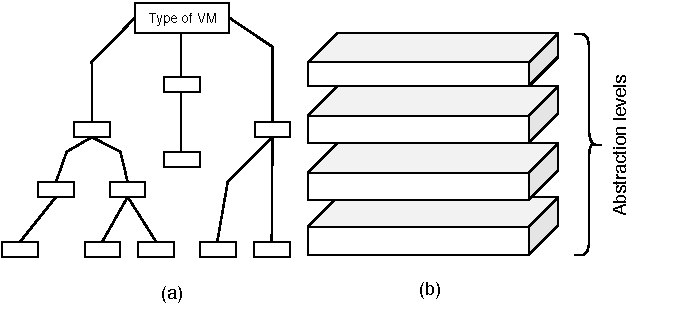
\includegraphics[width=8cm]{images/TwoApproaches.pdf}
%        %\vspace{1mm}
%        %\parbox[c]{8.3cm}{\footnotesize{Fig.1.~}  Example for inserting a one-column wide figure. }%\vspace*{.2mm}
%        \captionof{figure}{Two approaches used in the Taxonomy}
%        \label{fig:twoApproaches}
%    \end{center}

	\begin{figure}[H]
		\centering
		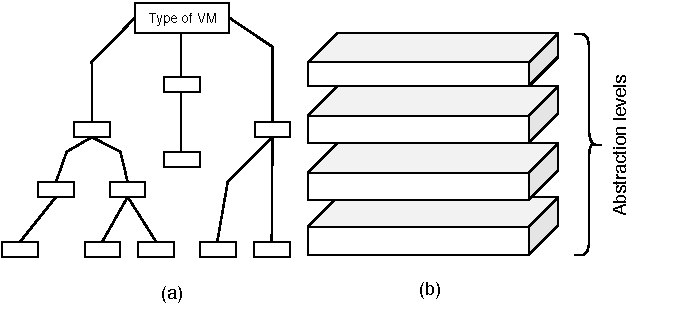
\includegraphics[width=8cm]{images/TwoApproaches.pdf}
		\vspace{-0.2cm}
		\caption{Two approaches used in the Taxonomy}
		\label{fig:twoApproaches}
	\end{figure}	
	
	The rest of the document is comprised of seven sections. Section \ref{sec:concetposVirtualizacion} introduces the basics of virtualization technologies.  Section \ref{sec:esquemasDeClasificacion} presents a description of previous classification schemes of virtualization technologies.  Section \ref{sec:necesidadDeUnaTaxonomia} describes the elements identified to propose a new taxonomy of virtual machines. Section \ref{sec:taxonomiaPropuesta} proposes a taxonomy that combines and updates the previous approaches. Section \ref{sec:choosingVirtualizationTechnology} presents a taxonomic diagram to guide the selection of the virtualization technologies identified in the proposed taxonomy.  Finally, Section \ref{sec:conclusion} presents our conclusions.
	
		\section {Virtualization concepts}\label{sec:concetposVirtualizacion}	
	
	This section presents some of the terms used in virtualization. 
	It begins with a general description of the concept of \textit{virtualization}, followed by the categories called \textit{elements} and \textit{virtualization techniques}.
	
	\subsection{Virtualization}
	
	%Virtualization is the combination of different technologies, which offer advantages to organizations. 
	Virtualization is a combination of technologies that can help with the management of large volumes of data, with rapid scalability of infrastructure and with effectively utilizing a shared set of massive computing capabilities. According to \textit{Kusnetzky} \cite{Kusnetzky2011}, virtualization makes it possible to make an abstraction of applications and underlying hardware components in a logical or virtual view of these resources \cite{AbdElRahem2016}. This virtual view can sometimes be noticeably different from the physical view of computing resources, such as processing power, memory, storage capacity or even network bandwidth \cite{Stallings2015}. In addition to the above, \textit{Silberschatz} \cite{Silberschatz2014} notes that virtualization is technology that allows operating systems to run as applications within other operating systems.
	
	%La virtualización también incluye el término \textit{emulación}, el cual es ampliamente conocido y hace referencia al hecho de tener diferencias entre la arquitectura base y la proyectada en el proceso de virtualización.
	
	%JNM  you could expand this a bit saying how a virtual machine could be the same architecture,  a variant of the same architecture with strategic modifications to make virtualization easier or a completely different architecture. 
	
	%LESR - old - Before JNM
	%Virtualization also includes the term \textit{emulation}, which is widely known and refers to the fact that there are differences between the base architecture and the architecture projected in the virtualization process.
	
	%LESR - new
	Virtualization also includes the term \textit{emulation}, which is widely known and refers to the fact that there are differences between the base architecture and the architecture projected in the virtualization process. That is, a virtual machine could have the same host architecture, a variant of the same architecture with strategic modifications to make virtualization easier or a completely different architecture.
	
	%Entre los objetivos de la virtualización se tiene: aumento de los niveles de rendimiento computacional, favorecer la escalabilidad y disponibilidad de sus soluciones tecnológicas de manera eficiente y eficaz, además de propender por unificar y usar de forma fácil las estructuras de administración y seguridad de la infraestructura computacional existente \cite{Kusnetzky2011}, \cite{Hui2014}. 
	
	%JNM not sure what you mean hear by "increasing the levels of computational performance"? do you mean increasing performance? or do you mean having different levels of abstraction?
	
	%LESR - new
	Some virtualization goals include increasing the levels of use of computational resources, favoring scalability and availability unifying and helping to use the administration and security structures of the existing computational infrastructure \cite{Kusnetzky2011}, \cite{Hui2014}.
	
	%JNM this paragraph seems quite clear to me  - good... the one above referencing Kusnetzky2011 and Hui2014 seemed less clear
	
	%LESR - new
	Through virtualization, it is possible to create a logical view that combines computational resources that can represent one or more operating environments. This means, for example, that many physical computers look like a single great resource (aggregation of resources) or, on the contrary, that a single machine is considered as several instances of itself (division of resources) \cite{Silberschatz2014}. Virtualization can take place using methodologies, such as partition or aggregation of hardware and software, partial or complete machine simulation, emulation and time sharing among others \cite{Chiueh2005}, \cite{Hoopes2009}. The separation of resources is one of the most common ways of using virtualization. In this case, it is possible to add the virtualization layer on top of real machine. This virtualization layer allows multiple virtualized environments to run simultaneously on the same real computer, either with the same architecture as the underlying system, with a variant of the same architecture including strategic modifications to facilitate virtualization, or with a completely different architecture for each particular need.
 

	
	%JNM Figure 1 and 3 were the same in the paper copy I have? Remove one?
	%\begin{figure}[!hbtp]
	%	\centering
	%	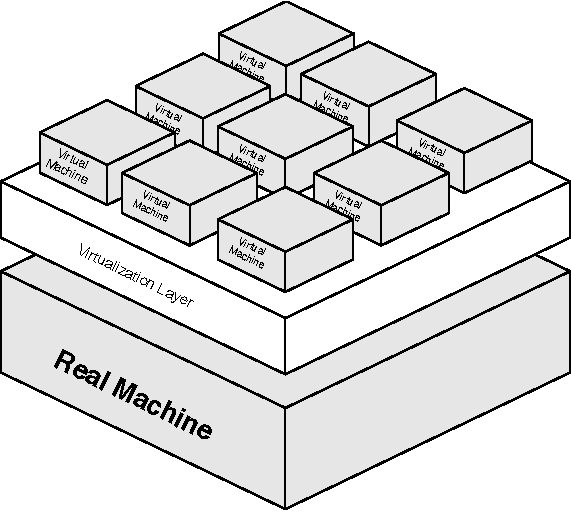
\includegraphics[width=7cm]{images/divisionRecursosFisicosConV12N.pdf}
	%	\vspace{-0.2cm}
	%	\caption{Division of resources through virtualization}
	%	\label{fig:divisionDeRecursosConVirtualizacion}
	%\end{figure}
	
	%JNM - this is also a place you could connect to the idea of virtualizing the same architecture, a variant of the same with strategic changes to make it easier to virtualize or completely different
	
	%LESR See above (Final part of the paragraph).
	
	Unfortunately, the x86 computer architecture, despite being one of the most widely adopted computer architecture in the world can not be virtualized completely\cite{Adams}. In this architecture, when executing instructions in non-privileged mode, some of them can fail silently instead of causing a trap and thus can not provide their respective treatment. 
	This situation can be solved through mechanisms and  virtualization approaches that act on different levels of abstraction. The abstraction levels where the virtualization takes place are the following: instruction set level, hardware abstraction level (HAL), operating system level (OS Level using system call interface), user-level library interface level and the application level \cite{Chiueh2005}. The virtualization concepts are grouped into the categories \textit{elements} and \textit{virtualization techniques}, which are described below.
	
	\subsection{Elements of virtualization}
	
	The elements \textit {real machine}, \textit {virtual machine} and \textit {virtual machine monitor}, are fundamental for understanding the virtualization technologies.
	These elements are described as follows.
	
	\subsubsection{Real machine}
	
	The term \textit{real machine} refers to the physical elements of the technological infrastructure that make up a computer; be it a personal computer, a workstation or a server. 
	Other references to this term are \textit {hardware}, \textit {physical hardware}, and \textit{bare-metal}. 
	In the commercial computer field, it is common to refer to the real machine concept using the word \textit{host} \cite{VMware2008}.
	
	\subsubsection{Virtual machine}
	
	The concept of \textit{virtual machine} (VM) is not new and was formalized in \textit{Goldberg}'s thesis in 1973 \cite {Goldberg1973} and published in various academic works in 1974 \cite{Popek1974}, \cite{Goldberg1974}. In these studies, virtual machine is defined as an efficient and isolated duplicate of the real machine, see Figure \ref{fig:TheVirtualMachineMonitor_Popek1974}. In later works, the term virtual machine has been extended to include other kinds of virtualization including applications at user level such as libraries, system calls, interfaces/services, system configurations, processes and state files \cite{Chiueh2005}. Another way of showing this concept is to relate to a software layer, which is put between the hardware or software resources and the applications \cite{Solis2014}. It is also very common in the commercial computing field to refer to the concept of VM using the word \textit{guest} \cite{VMware2008}. Finally, a virtual machine also is considered as an abstraction of computing resources presented as a service to allow them to operate simultaneously on the same real machine infrastructure \cite{Pek2013}.

%    \begin{center}
%		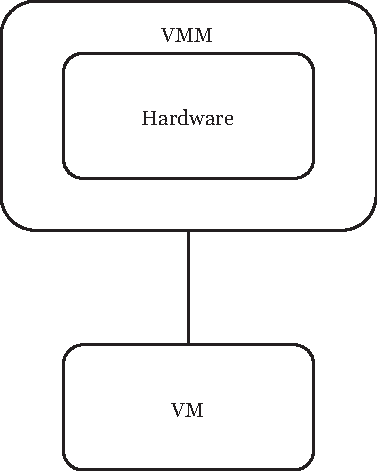
\includegraphics[width=3cm]{images/TheVirtualMachineMonitor_Popek1974.pdf}
%		\vspace{-0.2cm}
%        \captionof{figure}{Overview of virtual machine (VM) and virtual machine monitor (VMM)\footnotemark[2]{}.}
%        \label{fig:TheVirtualMachineMonitor_Popek1974}
%    \end{center}

	\begin{figure}[H]
		\centering
		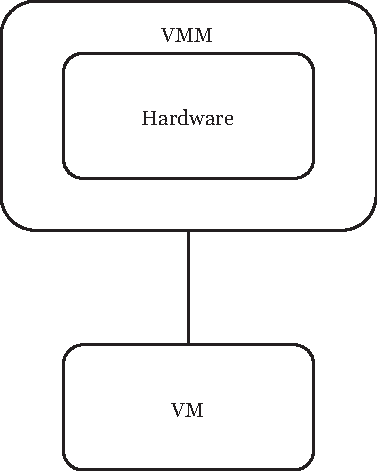
\includegraphics[width=3cm]{images/TheVirtualMachineMonitor_Popek1974.pdf}
		\vspace{0.2mm}
		\caption{Overview of virtual machine (VM) and virtual machine monitor (VMM) \cite{Popek1974}. }
		\label{fig:TheVirtualMachineMonitor_Popek1974}
	\end{figure}
	
	\subsubsection{Virtual machine monitor}
	
	The term \textit{virtual machine monitor} (VMM), was established by \textit{Popek} and \textit{Goldger} \cite{Popek1974}, in which they have defined the conceptual foundation of VMM as a piece of software that has three essential characteristics: \textbf{Equivalence}: To provide an execution environment for programs. This environment is identical to the original machine. \textbf{Performance}: Programs that run in this environment show, in the worst case, only minor decreases in speed. \textbf{Resource Control}: The VMM is in complete control of the system resources. The definition of a VMM is related to a software layer that provides support infrastructure using the resources of a lower level (usually \textit{hardware}), to create multiple VMs that are independent and isolated from each other \cite{Chiueh2005}, \cite{Cafaro2011}. Similarly, \textit{William Stallings} \cite{Stallings2015} determines that a VMM, is software that acts as an intermediary between the real machine and the VMs. 
	This software is commonly called \textit{Hypervisor} and it allows many VMs to coexist safely in the same hardware. The number of VMs that exist in a single computer determines the index of consolidation. In the particular case of Figure \ref{fig:VMM}, 9 to 1 is expressed as (9:1). The higher the consolidation index, the better the ROI and the less the TCO of the real machine used. Some of the functions and responsibilities of hypervisors are; emulation, isolation, resource allocation, and encapsulation \cite{Hoopes2009}.

%    \begin{center}
%		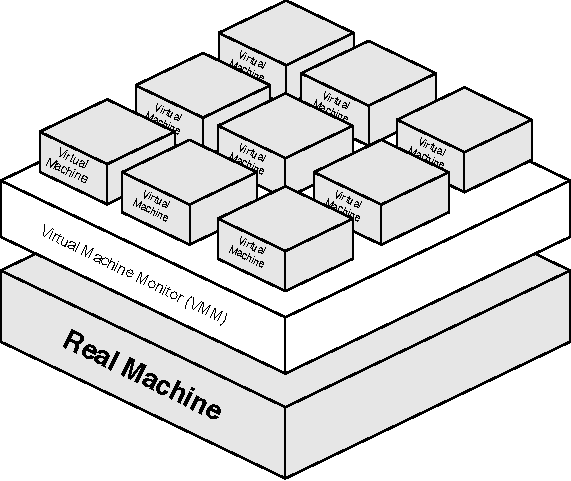
\includegraphics[width=6cm]{images/VMM.pdf}
%       %\vspace{1mm}
%        %\parbox[c]{8.3cm}{\footnotesize{Fig.1.~}  Example for inserting a one-column wide figure. }%
%        \vspace*{.2mm}
%        \captionof{figure}{Virtual Machine Monitor (VMM) or Hypervisor}
%        \label{fig:VMM}
%    \end{center}

    \begin{figure}[H]
        \centering
        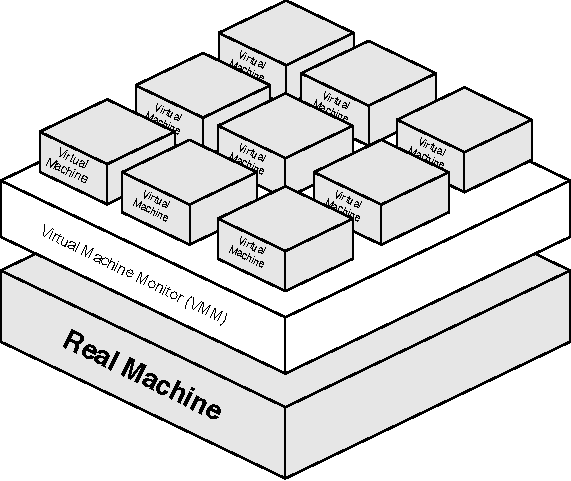
\includegraphics[width=6cm]{images/VMM.pdf}
        \vspace{0.2mm}
        \caption{Virtual Machine Monitor (VMM) or Hypervisor}
        \label{fig:VMM}
    \end{figure}

	\subsection{Virtualization techniques}
	
	The virtualization techniques called \textit{based on hypervisor} and \textit {based on containers} are described below. 
	These techniques are popular because they make it possible to consolidate hardware components easily.
	
	\subsubsection{Hypervisor-based virtualization technique}
	
	This virtualization technique consists of using the hypervisor as a central element, which takes in two different forms. The first one, is to locate the hypervisor directly onto the hardware. 
	This technique is also known as virtualization \textit{bare-metal} or \textit{native}, and the hypervisor is considered to be \textit{Type-1} (see Figure \ref{fig:Bare-metalHypervisor}). 
	The installation of this type of hypervisor does not need the presence of an underlying operating system. The second  form is to install the hypervisor on an existing operating system. 
	This technique is also known as virtualization \textit{hosted} or \textit{host-based}, and the hypervisor is considered to be \textit{Type-2} (see Figure \ref{fig:host-basedHypervisor}). 
	The main feature of Hypervisor-based virtualization is to create a fully operational virtual machine. This virtual machine can run independently and possibly on top of a different \textit{guest} operating systems, as long as they are compatible with delivered virtual architecture.

	\begin{figure}[H]
		\centering
		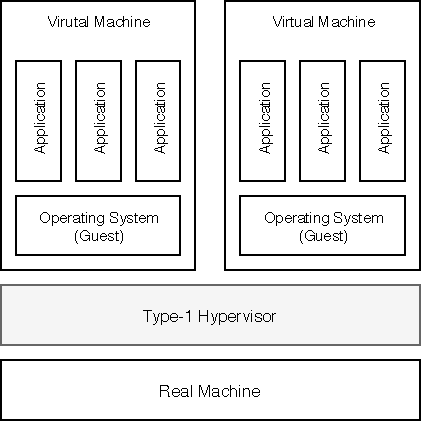
\includegraphics[width=6cm]{images/bare-metalHypervisor.pdf}
		\vspace{-0.2cm}
		\caption{Bare-metal Hypervisor}
		\label{fig:Bare-metalHypervisor}
	\end{figure}
	
	\begin{figure}[H]
		\centering
		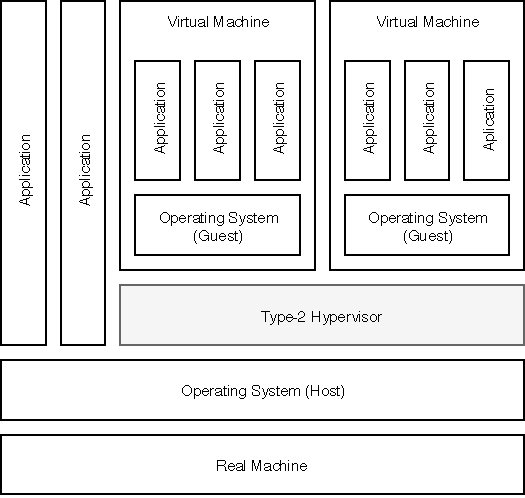
\includegraphics[width=6cm]{images/hosted-BasedHypervisor.pdf}
		\vspace{-0.2cm}
		\caption{Host-based hypervisor}
		\label{fig:host-basedHypervisor}
	\end{figure}
	
	\subsubsection {Container-based virtualization technique}
	
	This virtualization technique is based on a pre-existing operating system and consists of the generation of virtual execution environments for processes. 
	These execution environments are commonly called \textit{Containers} (see figure \ref{fig:container-baseVirtualization}). This virtualization technique requires fundamental parts of the OS to generate the virtual operating environments for the processes \cite{Kon2017}.
	Unlike hypervisor-based virtualization, which is required to generate VMs with whole operating systems,\cite{Kon2017}. 
	
	%This absence of OS supposes a lower computational load necessary to generate the virtual environment and in the same way, assumes that said environment is subject to the type of underlying operating system. 
	
	Avoiding the need for a separate OS in each container lowers the computational resources needed to support each container, but reduces flexibility because each container must have the same OS type and version. 

	\begin{figure}[H]
		\centering
		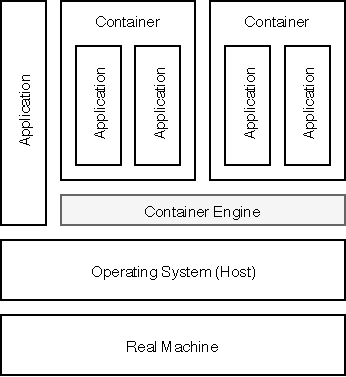
\includegraphics[width=6cm]{images/container-BasedVirtualization.pdf}
		\vspace{-0.2cm}
		\caption{Container-based virtualization}
		\label{fig:container-baseVirtualization}
	\end{figure}
	
		\section {Classification schemes for virtualization technologies}\label{sec:esquemasDeClasificacion}

    In this section, we survey existing classification schemes for virtualization technologies, highlighting their respective strengths and weaknesses.
    
    %Figure \ref{fig:TimeLine} presents some of these chronologically ordered approaches, which are described below.

%	\begin{figure}[H]%
%		\centering
%		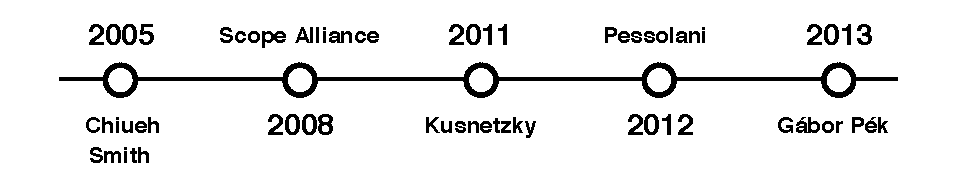
\includegraphics[width=8.5cm]{images/timeLine.pdf}
%		\vspace{-0.2cm} 
%		\caption{Classification schemes of virtualization technologies considered}
%		\label{fig:TimeLine}
%	\end{figure}
	
    	\subsection{Taxonomy of Virtualization Technologies by \textit{Chiueh}}

	\begin{figure}[!hbtp]
		\centering
		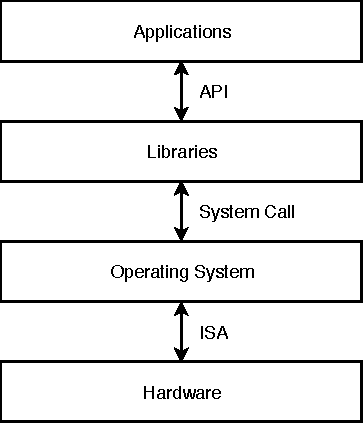
\includegraphics[width=4cm]{images/Chiueh2005.pdf}
		\vspace{-0.2cm}
		\caption{Levels of abstraction and virtualization application opportunities.\footnotemark[3]{}}
		\label{fig:VirtualizationOpportunities}
	\end{figure}
	
	\footnotetext[3]{Based on Figure 1 from the study \textit{A Survey on Virtualization Technologies} by Susanta Nanda Tzi-cker Chiueh, in 2005.}
	
	In the study, \textit{A Survery on Virtualization Technology} by \textit{Chiueh} in 2005 \cite{Chiueh2005}, a scheme is presented that's objective was to classify virtualization technologies according to the level of abstraction where they apply, see Figure \ref{fig:VirtualizationOpportunities}. Five levels are shown which correspond to \textit{Instruction Set Architecture Level}, \textit{Hardware Abstraction Layer}, \textit{Operating System Level}, \textit{Library Level} and \textit{Programming Language Level}. These levels of abstraction are described below.
	
	\subsubsection{Instruction Set Architecture Level} 
	
	This level includes the technologies relating to emulating the instruction set of the architecture in such a way that it is possible to provide a set of instructions different to the underlying hardware. This emulation implies the interpretation of the physical instructions through software. Examples of this type of technology are Bochs \cite{Bochs2018}, QEMU \cite {QEMU2018} and BIRD \cite {Nanda2006}.
	
	\subsubsection{Hardware Abstration Layer}
	
	This levels' virtualization technologies are based on abstractions that are between a real machine and an emulator. Here, the VM is an environment created and managed by a VMM, which in turn can manage VMs, in which it is possible to perform independent installations of operating systems, including their applications. These applications run as if they were executed in a real environment. Examples of these technologies are; VMware \cite{VMware2018Website}, Microsoft Virtual PC \cite{Honeycutt2003}, Denali \cite {Whitaker2002}, Xen \cite{Xen2018Website} \cite{Barham2003}, \cite{Xen2018WebsiteCambridge}, Plex86 \cite{Plex86}, Parallel \cite{Parallels2018} and UML \cite{Dike2006}, \cite{UML2006Website}. 
	
	\subsubsection{Operating System Level}
	
	This level is a virtualization tool that works through an operating system module to provide a virtualized system call interface,  such as; Jails \cite{Biederman2006} and Ensim \cite{Ensim}.
	
	\subsubsection{Library Level}
	
	At this level of abstraction, virtualization uses user-level libraries controlling the communication between the applications and the rest of the system. 
	That is to say, virtualization allows implementation as  an application binary interface (ABI) or an application programming interface (API). 
	For example, WINE \cite{Wine}, that allows supporting Windows applications on Unix-like systems. 
	Other examples are WABI \cite{WABI}, LXRun \cite{LXRUN} and Visual MainWin \cite{Fisher2006}.

	\subsubsection{Programming Language Level}
	
	This levels' virtualization technologies do not create a virtualization layer as an intermediary, but instead they implement the virtualization layer as an application that can create a virtual machine, which can be simple or complex, as is the case with the Java VM  (JVM) \cite{Lindholm1997}, Microsoft .NET common language infrastructure (CLI) \cite{Thai2003} and Parrot \cite {Parrot}. Although \textit{Chiueh} \cite{Chiueh2005} establishes an organized way to classify virtualization technologies, they do not consider the types of virtualization that exists at the same level of abstraction. In addition, it is necessary to include some technologies that have emerged in recent years.
    	\subsection{Virtual machine taxonomy by \textit{Smith and Nair}}
	
	\begin{figure}[!hbtp]
		\centering
		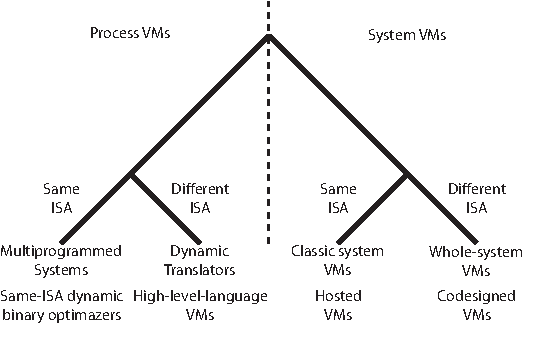
\includegraphics[width=8cm]{images/Smith2005.pdf}
		\vspace{-0.2cm}
		\caption{Virtual machine taxonomy proposed by Smith and Nair in 2005 \footnotemark [4]{}.}
		\label{fig:VMTaxonomySmithNair2005}
	\end{figure}
	
	\footnotetext[4]{Based on Figure 5 of \textit{The Architecture of Virtual Machines} by James E. Smith and Ravi Nair, in 2005.}
	
	In \textit{Smith} and \textit{Nair}'s study of 2005 \cite {Smith2005}, a taxonomy was presented that its objective was to classify the virtualization technologies into two large groups, such as, \textit{Process VMs} and \textit{System VMs}, see Figure \ref{fig:VMTaxonomySmithNair2005}. 
	
	%LESR - new
	 In general, it could be pointed out that the first level of division (Process vs. System) is about the level of virtualization but of coarser grain than that shown in the \textit{Chiueh's} study \cite{Chiueh2005}. The second level of decomposition refers to whether the virtual machine either Process or System is different from the underlying physical machine or not. 
    
    %JNM 
    System VMs contain an operating system and Process VMs instead access an underlying OS through an Application Binary Interface (ABI) or at the API level. In turn, each category is divided according to the execution or not of ISA simulations, giving rise to various subcategories which are explained below.
	
    %JNM - you could point out that Process vs System is about the level of virtualization but coarser grain than Chiueh2005 
    
    %JNM the second level of decomposition is about whether the virtual machine is different than the underlying physical machine or not
    
    %LESR - see above the new paragraph


	\subsubsection{Process VMs}
	
	The process VMs provide an environment in the ABI interface or at the API level. 
	It is called a multiprogrammed system when it uses the same ISA; otherwise, they are called dynamic emulators and binary translators. 
	The subcategories of the process virtual machines are described below:
	
%	\begin{itemize}		
%		\item \textbf{Multiprogrammed systems} reference the operating systems that implement multiprogramming through the management of timeshare access to the underlying hardware resources available. These systems use the same ISA and have the ability to handle multiple user processes "simultaneously." The operating system delivers an individual VM for each user process that runs concurrently. One implementation in this context are the \textit{Same-ISA dynamic binary optimizers} using the same ISA from the host system. Furthermore, these translators can make optimized translations of the code, an example of this technology is the Dynamo project \cite{Bala2011}.
		
%		\item \textbf{Dynamic translators} uses process VMs to support compiled binary programs for an ISA different from the underlying hardware. This implies executing an emulation effort performed through interpretation, which can be relatively slow. This situation can be compensated for through the \textit{dynamic binary translation} when a software cache is implemented to deal with the inherent overload of the binary translation. Examples of this implementation are the VMs of \textit{High-level languages} (HLL)  such as JVM \cite{Lindholm1997} or Microsoft .NET CLI Framework \cite{Fisher2006} \cite{Thai2003}.
%	\end{itemize} 

	\textbf{Multiprogrammed systems} reference the operating systems that implement multiprogramming through the management of timeshare access to the underlying hardware resources available. These systems use the same ISA and have the ability to handle multiple user processes "simultaneously." The operating system delivers an individual VM for each user process that runs concurrently. One implementation in this context are the \textit{Same-ISA dynamic binary optimizers} using the same ISA from the host system. Furthermore, these translators can make optimized translations of the code, an example of this technology is the Dynamo project \cite{Bala2011}.
		
	\textbf{Dynamic translators} uses process VMs to support compiled binary programs for an ISA different from the underlying hardware. This implies executing an emulation effort performed through interpretation, which can be relatively slow. This situation can be compensated for through the \textit{dynamic binary translation} when a software cache is implemented to deal with the inherent overload of the binary translation. Examples of this implementation are the VMs of \textit{High-level languages} (HLL)  such as JVM \cite{Lindholm1997} or Microsoft .NET CLI Framework \cite{Fisher2006} \cite{Thai2003}.

	
	\subsubsection{System VMs}
	
	These are characterized by hosting one or several complete and independent operating systems, running simultaneously on the same hardware of the host computer, as a result of the intermediation performed by the VMM. The subcategories of the system VMs are described below:
	
%	\begin{itemize}
	
%		\item \textbf{Classic system VMs} use the VMM and executes it directly on the bare hardware, that is to say, without the presence of an underlying operating system. The VMM  has real access to hardware resources and serves as an intermediary between the guest operating systems and the hardware itself. The VMs in this case are called \textit{Hosted VMs}.
		
%		\item \textbf{Whole-system VMs} provide virtualization of a complete environment, but unlike the previous category, guest systems use an ISA different from the one used in the underlying hardware. The VMs in this case are called \textit{Codesigned VMs}.
%	\end{itemize}

	\textbf{Classic system VMs} use the VMM and executes it directly on the bare hardware, that is to say, without the presence of an underlying operating system. The VMM  has real access to hardware resources and serves as an intermediary between the guest operating systems and the hardware itself. The VMs in this case are called \textit{Hosted VMs}.
		
	\textbf{Whole-system VMs} provide virtualization of a complete environment, but unlike the previous category, guest systems use an ISA different from the one used in the underlying hardware. The VMs in this case are called \textit{Codesigned VMs}.


	%JNM considered as a determinant?
	%LESR I changed "determinant" by "an important base"
	
	\textit{Smith} and \textit{Nair}'s study \cite{Smith2005} can be considered as an important base when classifying virtualization technologies in those that provide a virtual environment for a complete system or processes. However, this work does not contemplate what is established by \textit{Chiueh} \cite{Chiueh2005}, with regards to the levels of abstraction. Another important aspect is that this classification model does not have a high degree of detail, and in contrast, it uses a very general description level without even including particular technologies. It is important to consider that this study was carried out in 2005 and does not include technologies developed  subsequently.
	

    	\subsection{Virtualization taxonomy by \textit{SCOPE Alliance}}
	
	\begin{figure}[H]
		\centering
		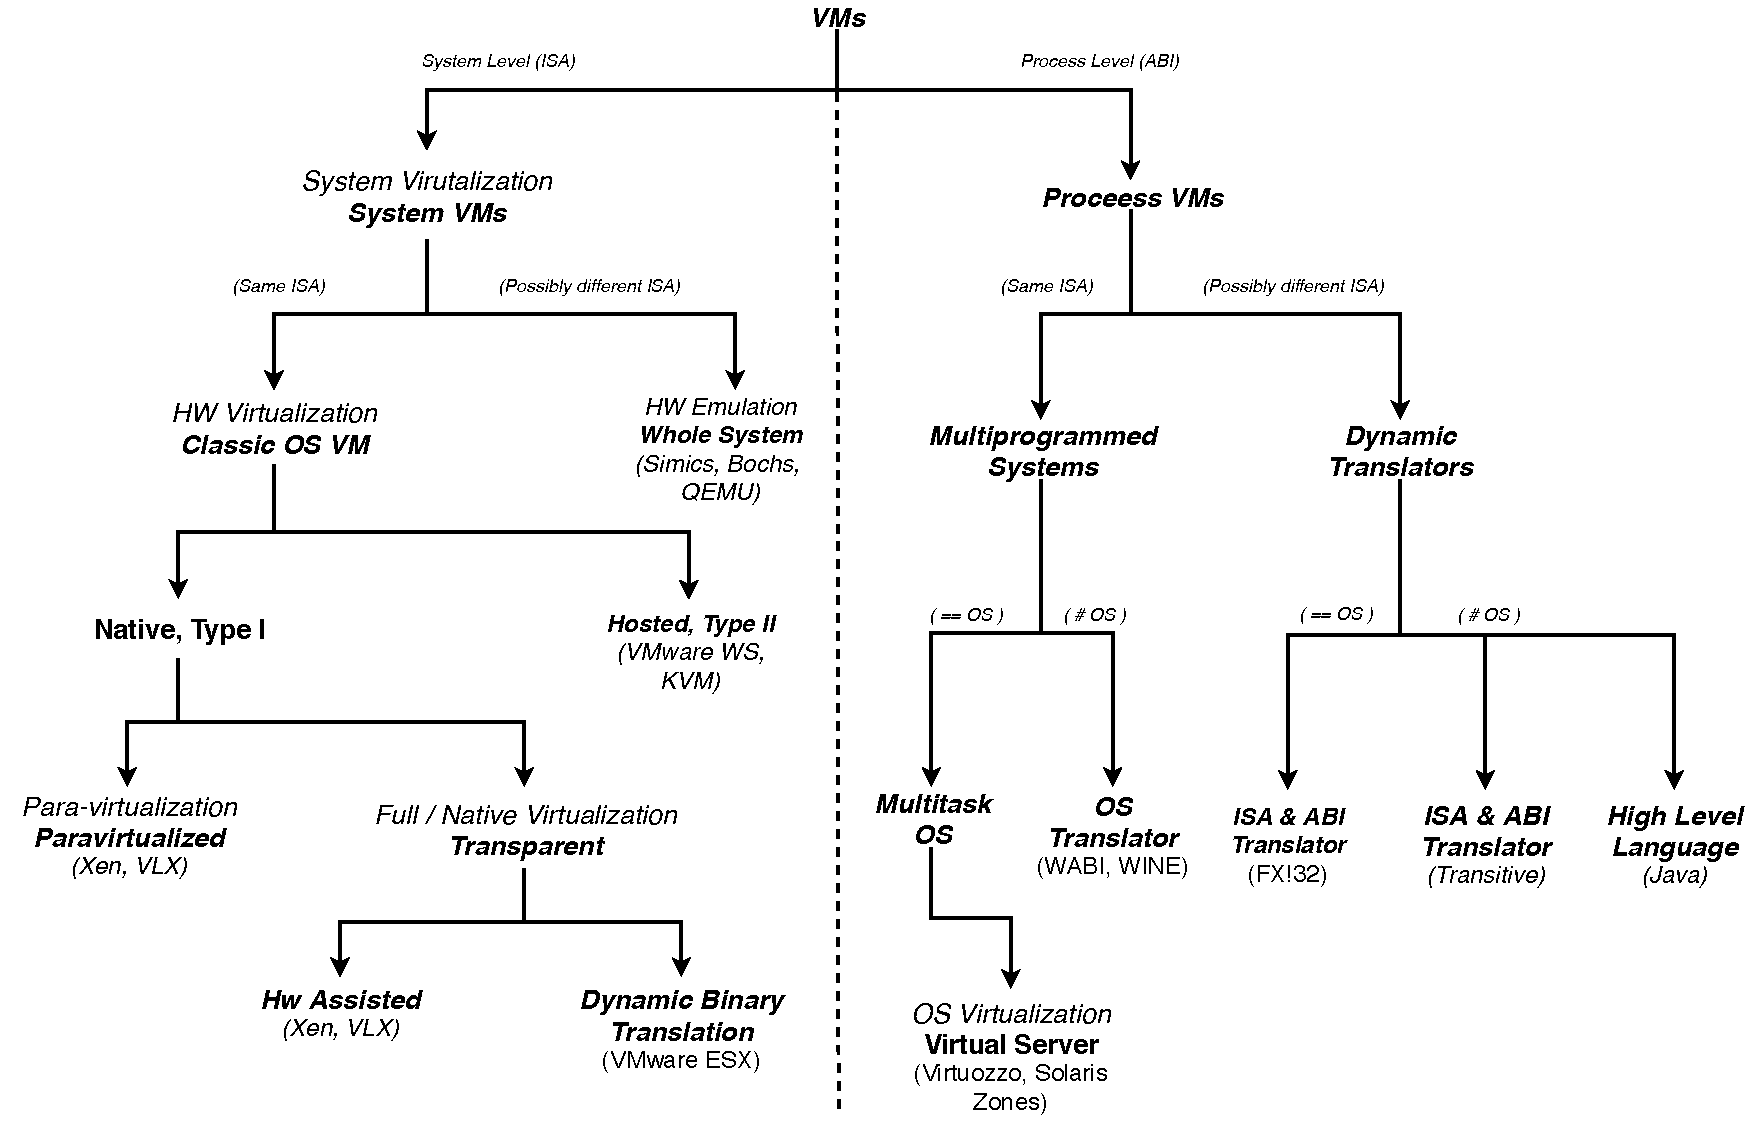
\includegraphics[width=8.5cm]{images/ScopeAlliance2008.pdf}
		\vspace{-0.2cm}
		\caption{Virtualization taxonomy by SCOPE Alliance Virtualization Working Group 2008 \cite{SCOPEAlliance2008}.}
		\label{fig:TaxonomyVirtualizationSCOPEAlliance2008}
	\end{figure}
	
    The group \textit{SCOPE Alliance Virtualization Working Group} 2008 proposed an extension of the work done  by \textit{Smith} and \textit{Nair} in 2005 \cite{Smith2005} \cite{SCOPEAlliance2008}. This classification also begins with a division into the high-level categories of systems or processes, but then each category is further broken down into smaller subcategories as shown in Figure \ref{fig:TaxonomyVirtualizationSCOPEAlliance2008}. 
	
	
	
	%With reference to the \textit{System VMs} (specifically with \textit{Whole system} and possibly different ISA) there are certain new elements such as, Simics \cite{Magnusson2002}, Bochs \cite{Bochs2018}, and QEMU \cite {QEMU2018}. 
	
	This classification places Type I and Type II hypervisors as distinctions of the \textit{Classic OS VM model} of System VMS that support the same ISA as the underlying hardware.  For Type I hypervisors, also know as \textit{Native}, it is also important to note that the taxonomy incorporates the concept of \textit{Para-virtualization} with examples, such as Xen \cite{Xen2018Website, Xen2018WebsiteCambridge}, VLX \cite{Armand2009} and the concept \textit{Full or native virtualization}. The latter can be seen either as \textit{Hardware Assisted}, such as, Xen and VLX,  or through \textit{Dynamic binary translation}, for instance, Vmware ESX. For Type II hypervisors, the examples of \textit{VMware Workstation} \cite{VMware2018Website} and KVM \cite{KVM} are also listed. 
	
	With reference to \textit{Process VMs} category, this classification distinguishes the \textit{Multiprogrammed System} and the \textit{Dynamic Translators}. \textit{Multiprogrammed Systems} are further classified depending on whether or not the OS provided by the underlying system is the same as the OS used by the application. If It is used the same OS, the category is called \textit{Multitask OS}, which in turn contain the category called \textit{OS Virtualization}, with examples such as \textit{Virtuozzo} \cite{OpenVZ, Virtuozzo} and \textit{Solaris Zones} \cite{SolarisZones}. If the OS is different, then the category is called \textit{Os Translator} and the taxonomy shows examples of technologies such as WABI and WINE. When the processes are possibly based on a different ISA, the category is called \textit{Dynamic Translators}. If the VMs use the same OS the category is called  \textit{ISA \& ABI Translator} for example, \textit{FX! 32} \cite{Chernoff1998}. If the OS is different, then there are two paths, the first is called \textit{ISA \& ABI Translator} for example \textit{Transitive} \cite {Transitive} and the second is called \textit{High-level Language} for example JAVA with its JVM.
	
	Although the \textit{SCOPE Alliance} study  \cite{SCOPEAlliance2008} constitutes a significant contribution along the way to complement the taxonomy of virtualization technologies; the research does not contemplate aspects of interest such as the levels of abstraction indicated by \textit{Chiueh} \cite{ Chiueh2005} in 2005. This situation gives rise to problems of conceptual inference, in which, for example, Type-1 and Type-2 hypervisors are perceived to be at the same level of abstraction. Additionally, according to the date of publication of the study, it is necessary to carry out an extension of concepts and an update of virtualization technologies that have emerged in recent years.
	
    	\subsection{Taxonomy of virtualization technologies by \textit{Kampert}}
	
	\begin{figure}[H]
		\centering
		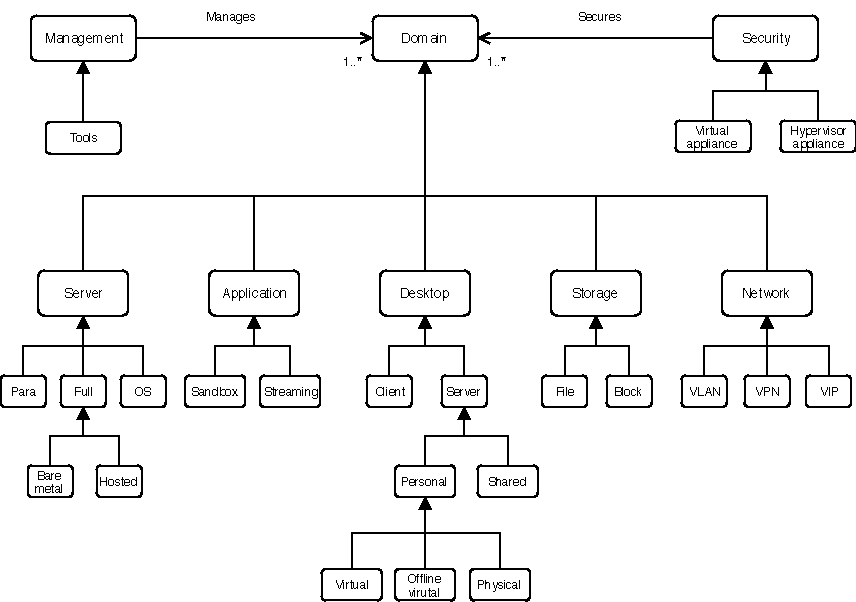
\includegraphics[width=8.5cm]{images/Kampert2010.pdf}
		\vspace{0.2mm}
		\caption{Kampert Taxonomy Model \cite{Kampert2010}.}
		\label{fig:KampertTaxonomyModel2010}
	\end{figure}
	
	In August 2010, \textit {Paulus Kampert} presented his Master's Degree dissertation called \textit{A Taxonomy of Virtualization Technologies} \cite{Kampert2010}. The objective of this work was to provide an overview of the different types of virtualization technologies and their trends. As a result, and with the sponsorship of the virtualization provider \textit{Atos Origin}, the taxonomy model developed shows the different layers of virtual server architecture and the virtualization domains in a structured way.
	
	The \textit{Kampert's} study of focused on the design of a taxonomy model to allow for the illustration of the different virtualization domains and their relationships. This model has been expressed using the Unified Modeling Language (UML), as shown in the Figure \ref{fig:KampertTaxonomyModel2010}.
	
	All elements of the model are called classes. \textit{Domain} is a superclass of the five domain classes: \textit{Server}, \textit{Application}, \textit{Desktop}, \textit {Storage} and \textit {Network}. The superclass in the center of the model facilitates the connection of the domain classes,
	these are \textit{Security} and \textit {Management}. These classes must apply to one or more virtualization domains. Additionally, each model's class can divide into a set of technologies. Below, each class is briefly described:

	\textbf{Server}:  Server virtualization can be divided into three subclasses such as \textit{Para-virtualization}, \textit{Full virtualization} and \textit{OS partitioning}. In turn, the \textit{Full virtualization} is divided into two more subclasses: \textit{Bare-metal} referring to \textit {Type-1 hypervisor} and \textit{Hosted} referring to \textit {Type-2 hypervisor}.
		
	\textbf {Application}: This domain comprises two subclasses corresponding to two types of application virtualization technologies: \textit{Sandbox} and \textit{Application Streaming}.
		
	\textbf{Desktop Virtualization}: Includes two types such as \textit{Client} and \textit{Server}. The \textit{Client desktop virtualization} is used to host virtual desktops (or VMs) on the client's computers. On the other hand, \textit{Server desktop virtualization} is divided into two types: \textit{Personal} and \textit{Shared}. \textit{Personal} is divided into \textit{Virtual}, \textit{Physical} and \textit{Offline virtual}.
		
	\textbf {Storage Virtualization}: Described as the data pool of multiple storage devices. This virtualization is divided into two classes,  \textit {Block virtualization} and \textit {File virtualization}. Examples of these technologies are SAN (\textit{Storage Area Network}) and NAS (Network Attached Storage).
		
	\textbf{Network Virtualization}: This domain comprises three types of technologies; such as, VLAN (LAN virtual), VIP (IP virtual) y VPN (Virtual Private Network).
		
    \textbf{Management}: Includes the five following technologies;  \textit{Performance}, \textit{Configuration}, \textit{Assets}, \textit{Capability} and \textit {Cost-control}.
		
	\textbf {Security}: Refers to the set of technologies developed specifically for virtualization. There are two types: \textit{Hypervisor appliance} and \textit{Virtual appliance}.
		
	\textit{Kampert}'s model intends to cover the domains in a more complete way in which the concept of virtualization takes place. The model itself does not offer the level of granularity necessary to identify particular types and technologies in each of the specified domains.

    	\subsection{Virtualization model by \textit{Kusnetzky}}
	
	\begin{figure}[H]
		\centering
		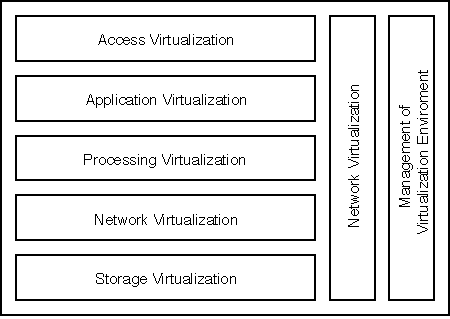
\includegraphics[width=8cm]{images/Kusnetzky2011.pdf}
		\vspace{-0.2cm}
		\caption{Kusnetzky Group model of virtualization \cite{Kusnetzky2011}.}
		\label{fig:kusnetzkyGroupModelOfVirtualization}
	\end{figure}
	
	In 2011, \textit{Dan Kusnetzky} presented the \textit{Virtualization Model of the Kusnetzky Group} \cite{Kusnetzky2011}, which aims to establish a way to organize  virtualizable computing resources, see Figure \ref{fig:kusnetzkyGroupModelOfVirtualization}. The model is composed of seven parts, five of them distributed in the form of layers or levels, located one above the other respectively. Each level represents a type of virtualization in a particular computing environment, such as: \textit{Access}, \textit{Application}, \textit{Processing}, \textit{Network} and \textit{Storage}. The two remaining parts correspond to the \textit{Security} and the \textit{Management} classes, arranged in parallel to the layers above. Below, each of them is briefly described:

	\textbf{Access virtualization} refers to the hardware and software that facilitate access to an application, making it possible for many users to share the same system.
		
	\textbf{Application virtualization} refers to software that allows applications to run transparently on different operating systems and hardware platforms.
		
	\textbf{Processing virtualization} includes the hardware and software elements that allow the division of resources (a system that appears to be many) or the aggregation of resources (many systems that appear to be one).

	\textbf{Network virtualization} refers to hardware and software technologies that make it possible to present a logical view of the physical network elements. This layer can be used for security and multiplexing purposes.
		
	\textbf{Storage virtualization} refers to hardware and software technologies that hide the location and type of physical storage devices in which applications store their data.
		
	\textbf{Security for virtual environment} refers to a set of software elements that make it possible to control access to the various elements of virtual media to protect them from unauthorized actions.
		
	\textbf{Management of virtual environment} refers to the software that makes it possible to performed the administrative and unified management of the available physical resources and the generated virtual environments.

	Although the \textit{Kusnetzky Group model of virtualization} presents a way to include categories for a range of virtualizable computational resources, the model does not provide a good level of detail about the existing technologies in each layer defined in the model. In addition, it does not differentiate between technologies of the same layer. For example, in the \textit{Processing virtualization} there is no evidence of a difference between the types of VMs present in Type-1 or Type-2 hypervisors. 
	
	It is important to note the date of the study and bear in mind technologies which have subsequently been developed. 

    	\subsection{Taxonomy of virtualization technologies by \textit{Pessolani}}
	
	\begin{figure}[H]
		\centering
		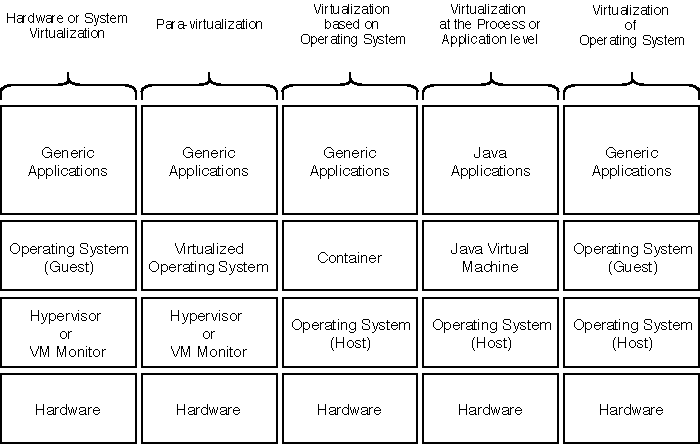
\includegraphics[width=8cm]{images/Pessolani2012.pdf}
		\vspace{-0.2cm}
		\caption{Taxonomy of virtual machines proposed by Pessolani et al in 2012 \cite{Pessolani2012}.}
		\label{fig:TaxonomiaDeTecnologiasDeVirtualizacion}
	\end{figure}
	
	Another way to distribute virtualization technologies is presented by \textit{Pessolani} and others in 2012 \cite{Pessolani2012}.  This study proposes a taxonomy with five main categories, such as; \textit{Hardware or System virtualization}, \textit{Para-virtualization}, \textit{Virtualization based on Operating}, \textit{Process or application-level virtualization} and \textit{Operating system virtualization}. See Figure \ref{fig:TaxonomiaDeTecnologiasDeVirtualizacion}. Additionally, layers are also displayed for each category, suggesting a level of abstraction in which each type of virtualization takes place. The categories of this taxonomy are described below:
	
		\textbf{Hardware or system virtualization} positions the Hypervisor (Type-1) directly on top of the hardware. This is where the VMs are located with their respective operating systems' \textit{guest} to support their applications.
		
		\textbf{Para-virtualization} distributes its elements similarly to hardware or system virtualization. However, in this case the operating system \textit{guest} has been modified to be aware that it is virtualized and take advantage of its condition.
		
		\textbf{Virtualization based on operating system} is based on the use of independent workspaces called \textit{Containers}, which are based on the operating system \textit{host}. These containers allow the execution of generic applications independently.
		
		\textbf {Virtualization at the process or application level} uses an application on the host operating system to provide a VM that allows the execution of processes based on that VM. For example, JVM and Java applications.
		
		\textbf {Operating system virtualization} needs an operating system \textit{host} which carries out the functions of a hypervisor to support the operating systems \textit{guests}, which in turn have their own completely independent applications. For example \textit{User Mode Linux} \cite{Dike2006} and \textit{Minix Over Linux} \cite{Pessolani2011}.

	
	Although \textit{Pessolani}'s  taxonomy presents a summarized form of grouping virtualization technologies, it does not  explicitly consider the level of abstraction in which these technologies apply. In addition, it focuses only on the conceptual elements leaving aside specific examples. Nor does it establish a way to divide types of VMs within each main category. In addition, according to the date of publication of the study, it is necessary to carry out an update of virtualization technologies that have emerged in recent years.
		\subsection{Taxonomy of virtualization concepts by \textit{P{\'e}k}}
	
	\begin{figure}[H]
		\centering
		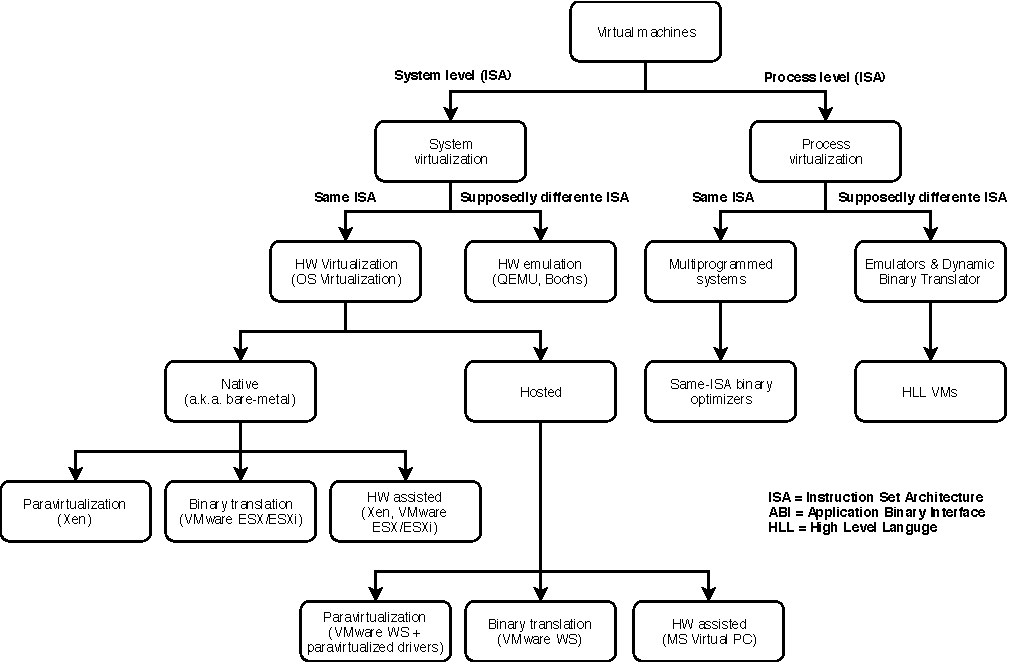
\includegraphics[width=8.5cm]{images/Pek2013.pdf}
		\vspace{-0.2cm}
		\caption{Taxonomy of virtualization concepts by \textit{G{\'a}bor P{\'e}k et al.} in 2013 \cite{Pek2013}.}
		\label{fig:TaxonomyOfVirtualizationConcepts}
	\end{figure}
	
	In 2013, \textit{P{\'e}k et al.} \cite{Pek2013} published research that includes a taxonomy of virtualization concepts. This study corresponds to an extension of the preliminary research by \textit{Smith} and \textit{Nair} in 2005 \cite{Smith2005}, and the \textit{SCOPE Alliance} in 2008 \cite {SCOPEAlliance2008}, see Figure \ref{fig:TaxonomyOfVirtualizationConcepts}. This contribution considers additional elements and the inclusion of several examples, particularly in the\textit{Hosted} category, which is equivalent to Type-2 hypervisors from the \textit{SCOPE Alliance} study. This taxonomy includes the subcategories of \textit{Para-virtualization} (VMware Workstation + Para-virtualization drivers), \textit{Binary translation} (VMware Workstation) and \textit{Hardware-assisted} (Microsoft Virtual PC). The other elements of the taxonomy follow the distribution originally proposed by the study of \textit{Smith} and \textit {Nair} in 2005. 
	
	Although \textit{P{\'e}k's} study presents a necessary extension to the previous research by the \textit{SCOPE Alliance} in 2008 \cite{SCOPEAlliance2008}, on the other hand, it shows a representation with less detail in the \textit{Process VMs} category, similar to \textit{Smit} and \textit{Nair}'s study in 2005 \cite{Smith2005}. Therefore, this taxonomy leaves a gap in the search for the details for the categorization of virtualization technologies. This is because, they are based on the above mentioned works, and they still have their limitations, since they do not contemplate the levels of abstraction in which virtualization technologies take place.
		\subsection{Taxonomy of virtualization by \textit{Ameen}}
	
	\begin{figure}[H]
		\centering
		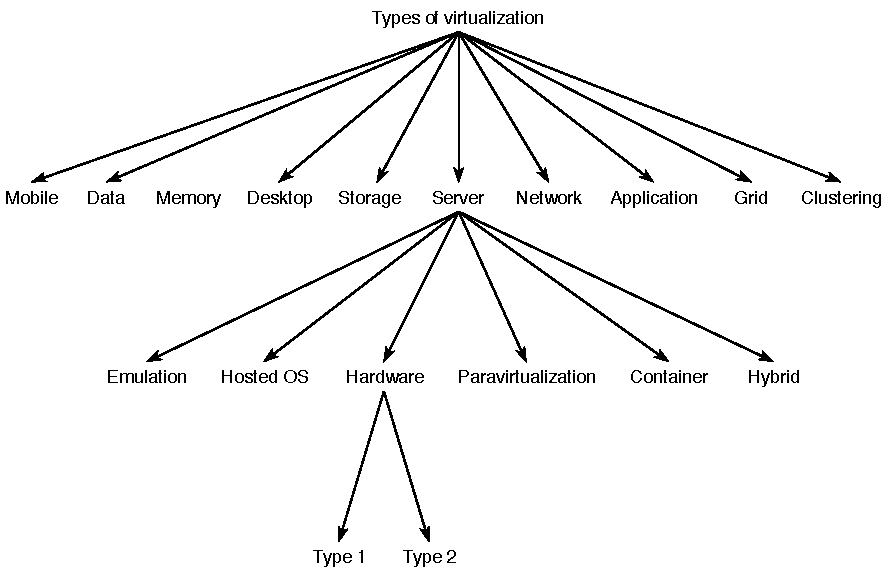
\includegraphics[width=8.5cm]{images/AmeenAndHamo2003.pdf}
		\caption{Taxonomy of virtualization by \textit{Ameen and A Hamo} \cite{Ameen2013}.} 
		\label{fig:TaxonomyOfVirtualizationByAmeen}
		%\vspace{1mm} 
	\end{figure}

%\noindent\rule{8.5cm}{0.4pt}
%		\vspace{1mm}
%	    \parbox[c]{8.5cm}{ \footnotesize Figure bases on the study \textit{A Survey of Server Virtualization} by Radhwan Y. Ameen and Asmaa Y. Hamo, in 2013}
%		\noindent\rule{8.5cm}{0.4pt}	    

%	\footnotetext [10]{Figure bases on the study \textit{A Survey of Server Virtualization} by Radhwan Y. Ameen and Asmaa Y. Hamo, in 2013.}

    From the perspective of the work of Ameen and Asmaa \cite{Ameen2013}, there are many different types of virtualization. In its first level is located some domains as  Mobile, Data, Memory, Desktop, Storage, Server, Network, Application, Grid and Clustering. Only Server virtualization is further decomposed. The second level shows the types considered for the Server Virtualization as Emulation, Hosted OS, Hardware, Paravirtualization, Container and Hybrid. Finally, the third level shows the types of virtualization considered for Hardware as Type 1 and Type 2. See Figure \ref{fig:TaxonomyOfVirtualizationByAmeen}.
    
    
    \textbf{Mobile virtualization} is a thin layer of software that is embedded on a mobile device to decouple the applications and data from the underlying hardware \cite{Ameen2013, VMware2018Website}. \textbf{Data virtualization} abstracts the source of individual data elements to allow applications to access data with a single methodology, regardless of how or where the data is stored \cite{Mann2006}. \textbf{Memory virtualization} consists of adding an extra level of address translation to give each VM the illusion of having zero memory address space, as provided by real hardware \cite{Ameen2013, Waldspurger2002}. \textbf{Desktop virtualization} is described as the ability to display a graphical desktop from one computer system on another computer system or device \cite{Ameen2013, VonHagen2008}. \textbf{Storage virtualization} is the emerging technology that creates logical abstractions of physical storage systems \cite{Ameen2013, Bigang2005}. \textbf{Server virtualization} is defined as the ability to run many operating systems with isolation and independence on other operating system \cite{Ameen2013}.
    \textbf{Network virtualization} provides an abstraction layer that can decouple the physical network equipment from the delivered business services over the network \cite{Annapareddy2011}. \textbf{Application virtualization} allows the user to run the application using local resources without installing the application in his system completely \cite{Annapareddy2011}. It also provides smaller single application virtual machines that allow for emulation of a specific environment on a client system.\cite{White2010}. \textbf{Grid virtualization} provides a way to abstract multiple physical servers (generally heterogeneous) from the application they are running \cite{Mann2006}. In \textbf{Clustering virtualization}, a cluster makes several locally-attached physical systems appear to the application and end users as a single processing resource \cite{Ameen2013, Mann2006}.
    
    Under the Server virtualization category,  \textbf{Emulation} is a virtualization method in which a complete hardware architecture may be created in software. This software is able to replicate the functionality of a designated hardware processor and associated hardware systems. \cite{Mann2006, Chiueh2005, VonHagen2008}.    \textbf{Hosted OS} virtualization is a software-only approach using a hypervisor layer that is hosted in an underlying operating system \cite{Ameen2013, VonHagen2008}. \textbf{Hardware} virtualization  is also referred to as hardware-assisted or full virtualization. Here the hypervisor is assisted by the processor hardware such as AMD-V or Intel VT-x processor virtualization technologies \cite{Ameen2013, VonHagen2008}. Hardware virtualization is further decomposed into  Type 1 and Type 2 hypervisors as we have seen in other classifications. 

    
    \textbf{Paravirtualization} refers to a technique in which the guest OS includes modified (paravirtualized) I/O drivers for the hardware. Unlike a binary translation approach, the hypervisor does not need to trap and translate all privileged layer instructions between the guest OS and the actual server hardware. Instead, the modified guest OS makes calls directly to the virtualized I/O services and other privileged operations \cite{Ameen2013, VonHagen2008}. \textbf{Container} virtualization is a kernel-layer abstraction and refers to  techniques in which the abstraction technology is built directly into the OS kernel rather than having a separate hypervisor layer \cite{Ameen2013, Lin2012}. Amen and Asmaa also includ the category \textbf{Hybrid}, referring to a combination of full virtualization and paravirtualization that uses input/output (I/O) acceleration techniques \cite{Ameen2013, White2010}.

    
    
    The Ammen and Asmaa's study is closely related to the works of Kampert \cite{Kampert2010} and Kusnetzky \cite{Kusnetzky2011} and presents a classification scheme through a three-level hierarchical structure. Although this graphical representation is simple and interesting, it is unbalanced because it focuses only on detailing the Server Virtualization category.




		\subsection{Taxonomy of Virtualization Tools by \textit{Abdulhamid}}
	
	\begin{figure}[H]
		\centering
		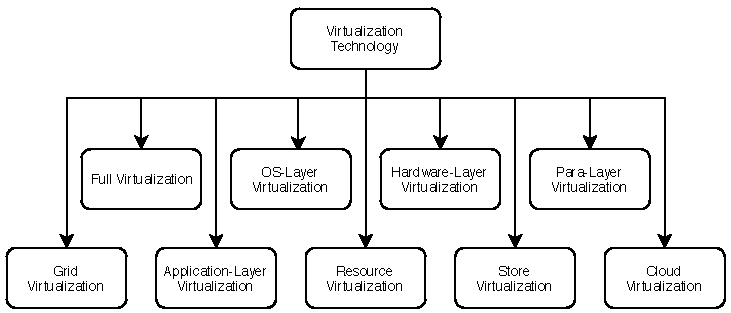
\includegraphics[width=8.5cm]{images/Abdulhamid2014.pdf}
		\vspace{-0.2cm}
		\caption{Taxonomy of virtualization tools by \textit{Shafi'i Muhammad Abdulhamid, Muhanmmad Shafie Abd Latiff and Mohammed Bakri Bashir} in 2014 \cite{Abdulhamid2014}.}
		\label{fig:TaxonomyByAbdulhamid}
	\end{figure}
	
	In the work of \textit{Abdulhamid} \cite{Abdulhamid2014} a taxonomy is presented whose purpose is to classify the hypervisors under the virtualization technology from the point of view of resource provisioning in cloud computing. This initiative is supported by the boom in cloud computing, particularly infrastructure as a service (IaaS). This purpose is based on the work of Sahoo, et al \cite{Sahoo2010}, which had the following seven categories: \textit{ Full Virtualization}, \textit{OS-Layer Virtualization}, \textit{Hardware-Layer Virtualization}, \textit{Para virtualization}, \textit{Application virtualization}, \textit{Resource virtualization}, \textit{Storage virtualization}. In addition, \textit{Abdulhamid's} work adds the followings two categories: \textit{Grid virtualization} and \textit{Cloud virtualization}. See Figure \ref{fig:TaxonomyByAbdulhamid}. Some of the categories proposed here have already been described, so below is brief description of the new terms.  
	
	\textbf{Resource virtualization} refers to the virtualization of a computer system such as storage volumes, name spaces and networks \cite{Abdulhamid2014}.	Some of the methods used to implement this type of virtualization include a) Combining several components in a larger pool of resources, b) Clusters of high-performance computers and c) Separating a resource many smaller resources.
	
	\textbf{Grid virtualization} focuses on virtualization of grid resources either for a Virtual Organization (VO) or for a Virtual Organization Cluster (VOC). The general aim is for hardware administrators to retain control of VMMs, as coarse grain resource sharing and monitoring can be executed by the grid.
	
	\textbf{Cloud virtualization} or cloud computing enables on-demand provisioning of virtual resources through the web and applying the concept of pay-per-use. Virtualization forms the basis of many cloud computing services, as it provides the ability to combine computing resources from clusters or networks and the provisioning of VM resources to customers on demand \cite{Abdulhamid2014, Aceto2013}.
	
	
	Although the work presented by \textit{Abdulhamid et al}. \cite{Abdulhamid2014} shows a graph suggesting two levels (See Figure \ref{fig:TaxonomyByAbdulhamid}), from a hierarchical perspective only one level can be observed comprising its nine categories. On the other hand, the description of each category lacks details and concrete examples of technologies that belong to each category described. 
	
	

		\subsection{Taxonomy of mobile virtualization techniques by \textit{Shuja}}
	
	\begin{figure}[H]
		\centering
		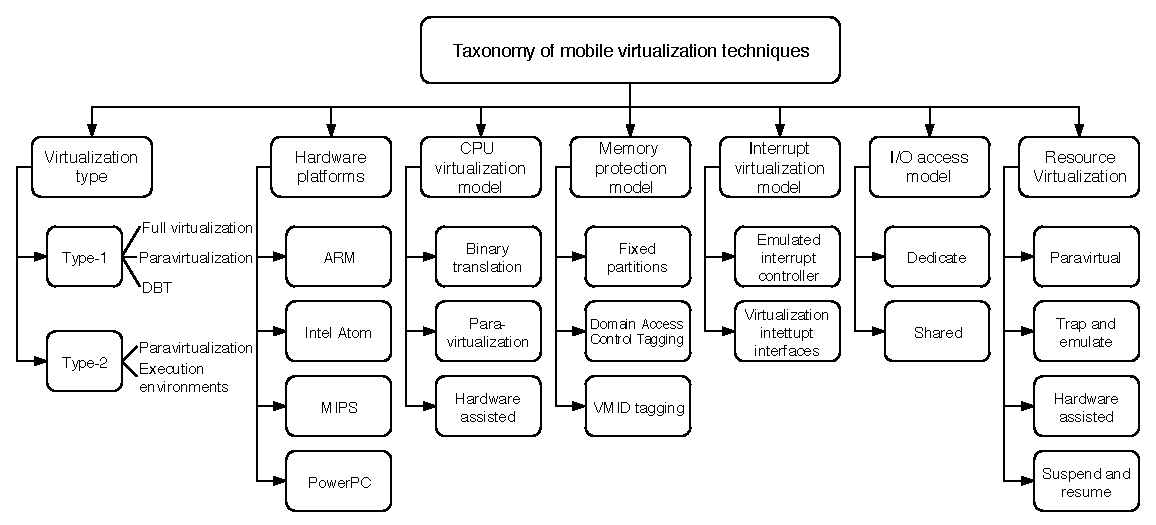
\includegraphics[width=8.5cm]{images/Shuja2016.pdf}
		\vspace{-0.2cm}
		\caption{Taxonomy of mobile virtualization techniques by \textit{Junaid Shuja, Kashif Bilal, Abdullah Gani and Samee Ullah Khan} in 2016 \cite{Shuja2016}.}
		\label{fig:TaxonomyByShuja}
	\end{figure}

	The study by Shuja et al \cite{Shuja2016} focuses on a taxonomy of mobile virtualization techniques with seven main categories: \textit{Virtualization type}, \textit{Hardware platforms}, \textit{CPU virtualization model}, \textit{Memory protection model}, \textit{Interrupt virtualization model}, \textit{I/O access model} and finally \textit{Network virtualization model}. 
	
	\textbf{Virtualization type} indicates the existence of two subcategories. As we have seen before, Type-1 is characterized by placing the guest OS directly on the underlying hardware and Type-2 by placing the guest OS on a underlying OS. \cite{Shuja2016, Zonghua2012}.
	
	\textbf{Hardware platform} presents the most popular manufacturers of infrastructure for mobile devices with are \textit{ARM}, \textit{Intel Atom}, \textit{MIPS}, and \textit{PowerPC}.
	
	\textbf{CPU virtualization model} shows different virtualization techniques such as \textit{Binary translation}, \textit{Paravirtualization} and \textit{Hardware assisted} virtualization used to trap and manage confidential instructions without privileges in ARM ISA. 
	
	\textbf{Memory protection model} shows three techniques such as Fixed partitions, Domain access control tagging, and VMID tagging. All of them focused on mobile devices with ARM ISA.

	\textbf{Interrupt virtualization model} shows that this process can be carried out using two techniques, either through "Emulated interrupt controller" or "Virtualization interrupt interfaces".

	\textbf{I/O access model} shows that it can be dedicated to a specific guest OS according to its priority or on the contrary, shared among all guest OSs. 

	\textbf{Network virtualization model} shows that it is possible to use four techniques such as: 1) \textit{Paravirtual} interfaces based on hypercalls, 2) \textit{Trap and emulate} procedure for network interface access, 3) \textit{Hardware assisted} multiple interface access to the guest OSs, and 4) \textit{Suspend and resume} routine. 
	
	Although Shuja et al.'s study \cite{Shuja2016} has considerable breadth in terms of the seven main categories discussed, they focus primarly on virtualization techniques for mobile devices, which limits the study's consideration of other important elements of the computing infrastructure.
	
	
	
	
	
	
	
	
	
	
	
	
	
	
		\subsection{Types of virtual machines by \textit{Xiao-Feng}}
	
	In the book called "\textit{Advanced Design and Implementation of Virtual Machines}" by Xiao-Feng in 2016 \cite{Xiao-Feng2016}, four types of virtual machines are presented:
	
	\textbf{Type 1}: The \textbf{Full ISA virtual machine} allows full ISA level emulation or virtualization. The operating system and its applications can run on top the VM as on a real machine\cite{Xiao-Feng2016}. Example VirtualBox, QEMU, and XEN.
	
	\textbf{Type 2}: The \textbf{ABI virtual machine} allows ABI-level emulation of the processes in the guest OS. There applications can run in conjunction with native ABI applications \cite{Xiao-Feng2016}. Example: Intel's IA-32 Execution Layer on Itanium, Transmeta's Code Morphing for X86 emulation.
	
	\textbf{Type 3}: The \textbf{Virtual ISA virtual machine} provides a runtime engine so that applications encoded in the virtual ISA can run on it \cite{Xiao-Feng2016}. Example Sun Microsistem's JVM, Microsoft's Common Language Runtime, and Parrot Foundation's virtual machine \cite{Parrot}.
	
	\textbf{Type 4}: The \textbf{Language virtual machine} gives a runtime engine that runs programs written in a guest language (source). The runtime engine needs to interpret or translate the program. Example, the runtime engines for Basic, Lisp, Tcl, and Ruby.
	
	Although the study by Xiao-Feng et al. presents a classification scheme of four types, its does not indicate a hierarchical structure that clarifies how they relate. It also does not have a supporting graph to facilitate understanding. They also do not contemplate many of the categories indicated in other taxonomies previously presented.
	
	
		\subsection{Taxonomy of virtualization by \textit{Bugnion}}
	
	\begin{figure}[H]
		\centering
		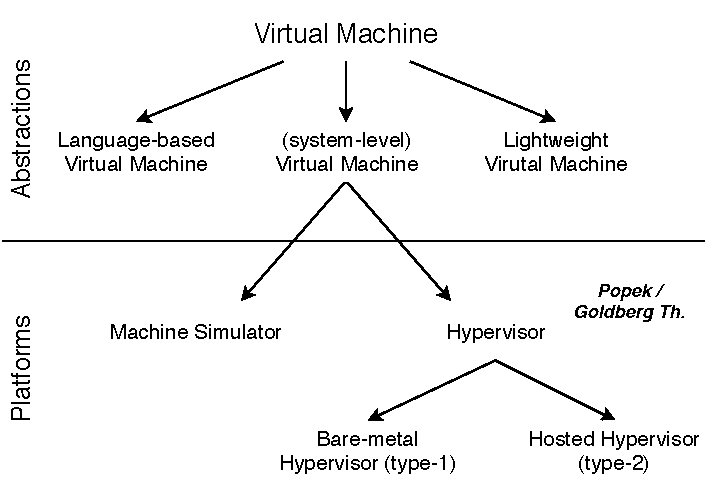
\includegraphics[width=8.5cm]{images/Bugnion2017.pdf}
		\vspace{-0.2cm}
		\caption{Basic classification of virtual machines and the platforms that run them by \textit{Edouard Bugnion, Jason Nieh, Dan Tsafrir and Margaret Martonosi} in 2017 \cite{Bugnion2017}.}
		\label{fig:TaxonomyOfVirtualizationBugnion}
	\end{figure}
	   
    In the \textit{Bugnion et al.}'s book \cite{Bugnion2017}  presents an interesting structure with two level that show the concepts related with the VMs. The first level is related with \textit{Abstraction} and its include the categories \textit{Language-base VM}, \textit{System-level VM}, and \textit{Lightweight VM}. The second level is related with \textit{Platform} and its include two categories derivative from \textit{System-level VM} called \textit{Machine Simulator}, and \textit{Hypervisor}. The latter, is divided in \textit{Bare-metal Hypervisor} also called \textit{Type-1}, and \textit{Hosted Hypervisor} also called \textit{Type-2}.
    
    \textbf{Language-based VMs} refers to the run-time environment of any managed language such as the Java Virtual Machine, Microsoft Common Language Runtime, and Javascript engines embedded in browsers.  
    
    \textbf{Lightweight VMs} refers to software mechanisms to ensure that applications run directly on the processor as securely isolated from other environments and the underlying OS. This includes examples such as Denali \cite {Whitaker2002}, Google Native Client \cite{Yee2009}, Vx32 \cite{Ford2008}, Docker \cite{Docker} y FreeBSD Jail \cite{Kamp2000}.
    
    \textbf{System-level VMs} refers to the computer environment resembles the hardware of a computer so that the VM can run an OS and its applications, in full isolation from the other virtual machines and the rest of the environment.  This category includes two types (type-1 and type2) of Hypervisor but they were already described before in this document.
    
    \textit{Bugnion et al.} is less a taxonomy than a book focusing on the core architectural support that must be provided by hardware to efficiently run virtual machines.
%	Although in the \textit{Bugnion et al.}'s study \cite{Bugnion2017} there is an interesting way to classified VMs when presenting Platform / Abstractions separation. However, the level of detail presented is superficial and leaves out of consideration many other elements that are part of virtualization technologies.
	
	

	                                                                                                                                                                                                                                                                                                                                                                                                                                                                                                                                                                                                                                                                                                                                                                                                                                                                                                                                                                                                                                                                                                                                                                                                                                                                                                                                                                                                                                                                                                                                                                                                                                                                                                                                                                                                                                                                                                                                                                                                                                                                                                                                                                                                                                                                                                                                                                                                                                                                                                                                                                                                                                                                                                                                                                                                                                                                                                                                                                                                                                                                                                                                                                                                                                                                                                                                                                                                                                                                                                                                                                                                                                                                                                                                                                                                                                                                                                                                                                                                                                                                                                                                                                                                                                                                                                                                                                                                                                                                                                                                                                                                                                                                                                                                                                                                                                                                                                                                                                                                                                                                                                                                                                                                                                                                                                                                                                                                                                                                                                                                                                                                                                                                                                                                                                                                                                                                                                                                                                                                                                                                                                                                                                                                                                                                                                                                                                                                                                                                                                                                                                                                                                                                                                                                                                                                                                                                                                                                                                                                                                                                                                                                                                                                                                                                                                                                                                                                                                                                                                                                                                                                                                                                                                                                                                                                                                                                                                                                                                                                                                                                                                                                                                                                                                                                                                                                                                                                                                                                                                                                                                                                                                                                                                                                                                                                                                                                                                                                                                                                                                                                                                                                                                                                                                                                                                                                                                                                                                                                                                                                                                                                                                                                                                                                                                                                                                                                                                                                                                                                                                                                                                                                                                                                                                                                                                                                                                                                                                                                                                                                                                                                                                                                                                                                                                                                                                                                                                                                                                                                                                                                                                                                                                                                                                                                                                                                                                                                                                                                                                                                                                                                                                                                                                                                                                                                                                                                                                                                                                                                                                                                                                                                                                                                                                                                                                                                                                                                                                                                                                                                                                                                                                                                                                                                                                                                                                                                                                                                                                                                                                                                                                                                                                                                                                                                                                                                                                                                                                                                                                                                                                                                                                                                                                                                                                                                                                                                                                                                                                                                                                                                                                                                                                                                                                                                                                                                                                                                                                                                                                                                                                                                                                                                                                                                                                                                                                                                                                                                                                                                                                                                                                                                                                                                                                                                                                                                                                                                                                                                                                                                                                                                                                                                                                                                                                                                                                                                                                                                                                                                                                                                                                                                                                                                                                                                                                                                                                                                                                                                                                                                                                                                                                                                                                                                                                                                                                                                                                                                                                                                                                                                                                                                                                                                                                                                                                                                                                                                                                                                                                                                                                                                                                                                                                                                                                                                                                                                                                                                                                                                                                                                                                                                                                                                                                                                                                                                                                                                                                                                                                                                                                                                                                                                                                                                                                                                                                                                                                                                                                                                                                                                                                                                                                                                                                                                                                                                                                                                                                                                                                                                                                                                                                                                                                                                                                                                                                                                                                                                                                                                                                                                                                                                                                                                                                                                                                                                                                                                                                                                                                                                                                                                                                                                                                                                                                                                                                                                                                                                                                                                                                                                                                                                                                                                                                                                                                                                                                                                                                                                                                                                                                                                                                                                                                                                                                                                                                                                                                                                                                                                                                                                                                                                                                                                                                                                                                                                                                                                                                                                                                                                                                                                                                                                                                                                                                                                                                                                                                                                                                                                                                                                                                                                                                                                                                                                                                                                                                                                                                                                                                                                                                                                                                                                                                                                                                                                                                                                                                                                                                                                                                                                                                                                                                                                                                                                                                                                                                                                                                                                                                                                                                                                                                                                                                                                                                                                                                                                                                                                                                                                                                                                                                                                                                                                                                                                                                                                                                                                                                                                                                                                                                                                                                                                                                                                                                                                                                                                                                                                                                                                                                                                                                                                                                                                                                                                                                                                                                                                                                                                                                                                                                                                                                                                                                                                                                                                                                                                                                                                                                                                                                                                                                                                                                                                                                                                                                                                                                                                                                                                                                                                                                                                                                                                                                                                                                                                                                                                                                                                                                                                                                                                                                                                                                                                                                                                                                                                                                                                                                                                                                                                                                                                                                                                                                                                                                                                                                                                                                                                                                                                                                                                                                                                                                                                                                                                                                                                                                                                                                                                                                                                                                                                                                                                                                                                                                                                                                                                                                                                                                                                                                                                                                                                                                                                                                                                                                                                                                                                                                                                                                                                                                                                                                                                                                                                                                                                                                                                                                                                                                                                                                                                                                                                                                                                                                                                                                                                                                                                                                                                                                                                                                                                                                                                                                                                                                                                                                                                                                                                                                                                                                                                                                                                                                                                                                                                                                                                                                                                                                                                                                                                                                                                                                                                                                                                                                                                                                                                                                                                                                                                                                                                                                                                                                                                                                                                                                                                                                                                                                                                                                                                                                                                                                                                                                                                                                                                                                                                                                                                                                                                                                                                                                                                                                                                                                                                                                                                                                                                                                                                                                                                                                                                                                                                                                                                                                                                                                                                                                                                                                                                                                                                                                                                                                                                                                                                                                                                                                                                                                                                                                                                                                                                                                                                                                                                                                                                                                                                                                                                                                                                                                                                                                                                                                                                                                                                                                                                                                                                                                                                                                                                                                                                                                                                                                                                                                                                                                                                                                                                                                                                                                                                                                                                                                                                                                                                                                                                                                                                                                                                                                                                                                                                                                                                                                                                                                                         
    	\section {Need for a new taxonomy}\label{sec:necesidadDeUnaTaxonomia}
	
	The set of taxonomies described above have many elements that contribute to the classification of virtualization technologies. However, in each of these classification schemes aspects which need to be improved have been identified. On the other hand, each scheme offers a taxonomic approach, such as a) \textit{Abstraction level}, b) \textit{Type of VM} and c) \textit{Virtualization domains}. Table \ref{cuadro:resumenTrabajos} shows a summary of the classification schemes analyzed in this paper, which are identified by; author, year of publication and taxonomic approach. This table describes taxonomies published between 2005 and 2017. It is worth noting that we found no taxonomies published in 2018 or 2019.
	
	%JNM - are you planning to add 2013-2018? do you have a list of other taxonomies proposed in that time?  If so I think you have to cover those to have a viable paper. 
	
	%LESR I have already finished it. Please, see following sections: 3.8 Ammen, 3.9 Abdulhamid, 3.10 Shuja, 3.11 Xiao-Feng Li and 3.12 Bugnion.
	
	\begin{table}[H]
		\centering
		\begin{tabular}{|l|c|p{3.9cm}|}
			\hline
			\multicolumn{3}{|c|}{\textbf{Classification schemes analyzed}}\\
			\hline
			\textbf{Author} & \textbf{Year} & \textbf{Taxonomic approach} \\ 
			\hline
			Chiueh          & 2005          & Abstraction level\\ 
			\hline
			Smith           & 2005          & Type of VM\\ 
			\hline
			Scope Alliance  & 2008          & Type of VM\\ 
			\hline
			Kampert         & 2010          & Virtualization Domains\\ 
			\hline
			Kusnetzky       & 2011          & Virtualization Domains\\ 
			\hline
			Pessolani       & 2012          & Type of VM\\ 
			\hline
			P{\'e}k         & 2013          & Type of VM\\ 
			\hline
			Ameen           & 2013          & Type of VM and Virtualization Domains\\ 
			\hline
			Abdulhamid      & 2014          & Type of VM and Virtualization Domains\\ 
			\hline
			Shuja           & 2016          & Type of VM\\ 
			\hline
			Xiao-Feng Li    & 2016          & Abstraction level\\ 
			\hline
			Bugnion         & 2017          & Type of VM and Abstraction levels\\ 
			\hline
		\end{tabular}
		\caption{Summary of classification schemes}
		\label{cuadro:resumenTrabajos}
		
	\end{table}

    %LESR new
	The taxonomic approach \textit{Type of VM} is the most popular taxonomic approach, as demonstrated by the studies of \textit{Smith and Nair}, \textit{SCOPE Alliance Virtualization Working Group} \cite{SCOPEAlliance2008}, \textit{Pessolani et al.} \cite{Pessolani2012}, \textit{P{\'e}k} \cite{Pek2013}, and \textit{Shuja et al.} \cite{Shuja2016}. On the other hand, \textit{Kampert} \cite{Kampert2010} and \textit{Kusnetzky} \cite{Kusnetzky2011} take a different perspective, that's objective is to consider in a general way, the largest number of technological domains in which it is possible to carry out virtualization processes, hence the name \textit{Virtualization domains}. Some taxonomies can be perceived as dual approach, for example the studies by \textit{Ammen et al.} \cite{Ameen2013} and \textit{Abdulhamid et al.} \cite{Abdulhamid2014} combine \textit{Type of VM} with \textit{Domains}, and the \textit{Bugnion et al.}'s study \cite{Bugnion2017} combine \textit{Type of VM} with \textit{Abstraction level}. Lastly, \textit{Chiueh} \cite{Chiueh2005} and \textit{Xiao-Feng et al.} \cite{Xiao-Feng2016} consider the taxonomic approach \textit{Abstraction level} as fundamental for the categorization of virtualization technologies. When there are differences in approach to these issues, interested communities may feel confused when they are reading different authors. This is why there is a need for a taxonomy that provides a unified, organized and updated view for this topic.
	
	%JNM Refuerce esto si puede con más información sobre lo que hace su propuesta además de los objetivos. ¿Qué nuevos elementos se agregan por ejemplo?

	%LESR old
	%This new taxonomy should combine approaches and add new elements. This new taxonomy should be an instrument to provide support in pedagogical processes and learning in the academic community with interests in virtualization technologies. On the other hand, the new taxonomy should also facilitate the visualization of the technological ecosystem that surrounds this topic. It should help industry in its decision-making processes for the selection of these types of technologies.
	

	%JNM Creo que es una contribución reunir todas las taxonomías existentes y compararlas. ¿No tendría que argumentar que una nueva es necesaria, solo que está ubicando las existentes en un contexto para poder compararlas?
	
	%JNM Eso podría ser un argumento más fácil. ¿No es que ha habido muy pocas taxonías, pero que ha habido demasiadas y que está haciendo el trabajo de compararlas y ponerlas en contexto entre sí?
	
	
	%Creo que esta podría ser una mejor manera de posicionar las contribuciones que como una nueva taxonomía.
	
	
	% JNM tambine estan contribuyendo una visualización que los pone en contexto y un diagrama de flujo basado en esto para ayudar en la selección de tecnologías de virtualización apropiadas en un espacio confuso.
	

    %LESR I tried to give answer to all questions wrote above with the follow 
    
In this paper, We make the following three contributions:

    1) A study that corresponds to the review of the literature that included the identification, analysis, characterization and comparison of twelve classification schemes on virtual machines and/or virtualization technologies. See section \ref{sec:esquemasDeClasificacion}. The set of studies considered is summarized in table \ref{cuadro:resumenTrabajos}. 

    2) Construction of a new Virtual Machine Taxonomy proposal, in the process of which some of the existing studies were identified, expanded and combined, which allows offering in a single image the visualization of multiple concepts related to the types of virtual machines and the respective level of abstraction where they are performed in relation to the classical architecture of a computer system. See Figure \ref{fig:TaxonomiaPropuesta}.  The proposed taxonomy includes examples of older virtualization technologies, in order to provide a reference factor to those who have some knowledge about them. It also includes examples of new virtualization technologies that have gained wide recognition in industry and academia, such as those related to containers. In addition, the taxonomy is also intended to be an instrument to support the pedagogical processes of teaching and learning in the academic community with interests in virtualization technologies. 

    3) Elaboration of a taxonomic-key diagram whose purpose is to facilitate the visualization of the technological ecosystem that surrounds this topic and, consequently, to help the academic and industrial community in the decision making processes for the selection of this type of technologies. See Figure \ref{fig:taxonomic-keyDiagram}.
    	\section {Virtual Machine Taxonomy Proposal} \label{sec:taxonomiaPropuesta}
	
	\begin{figure*}[ht]
		\centering
		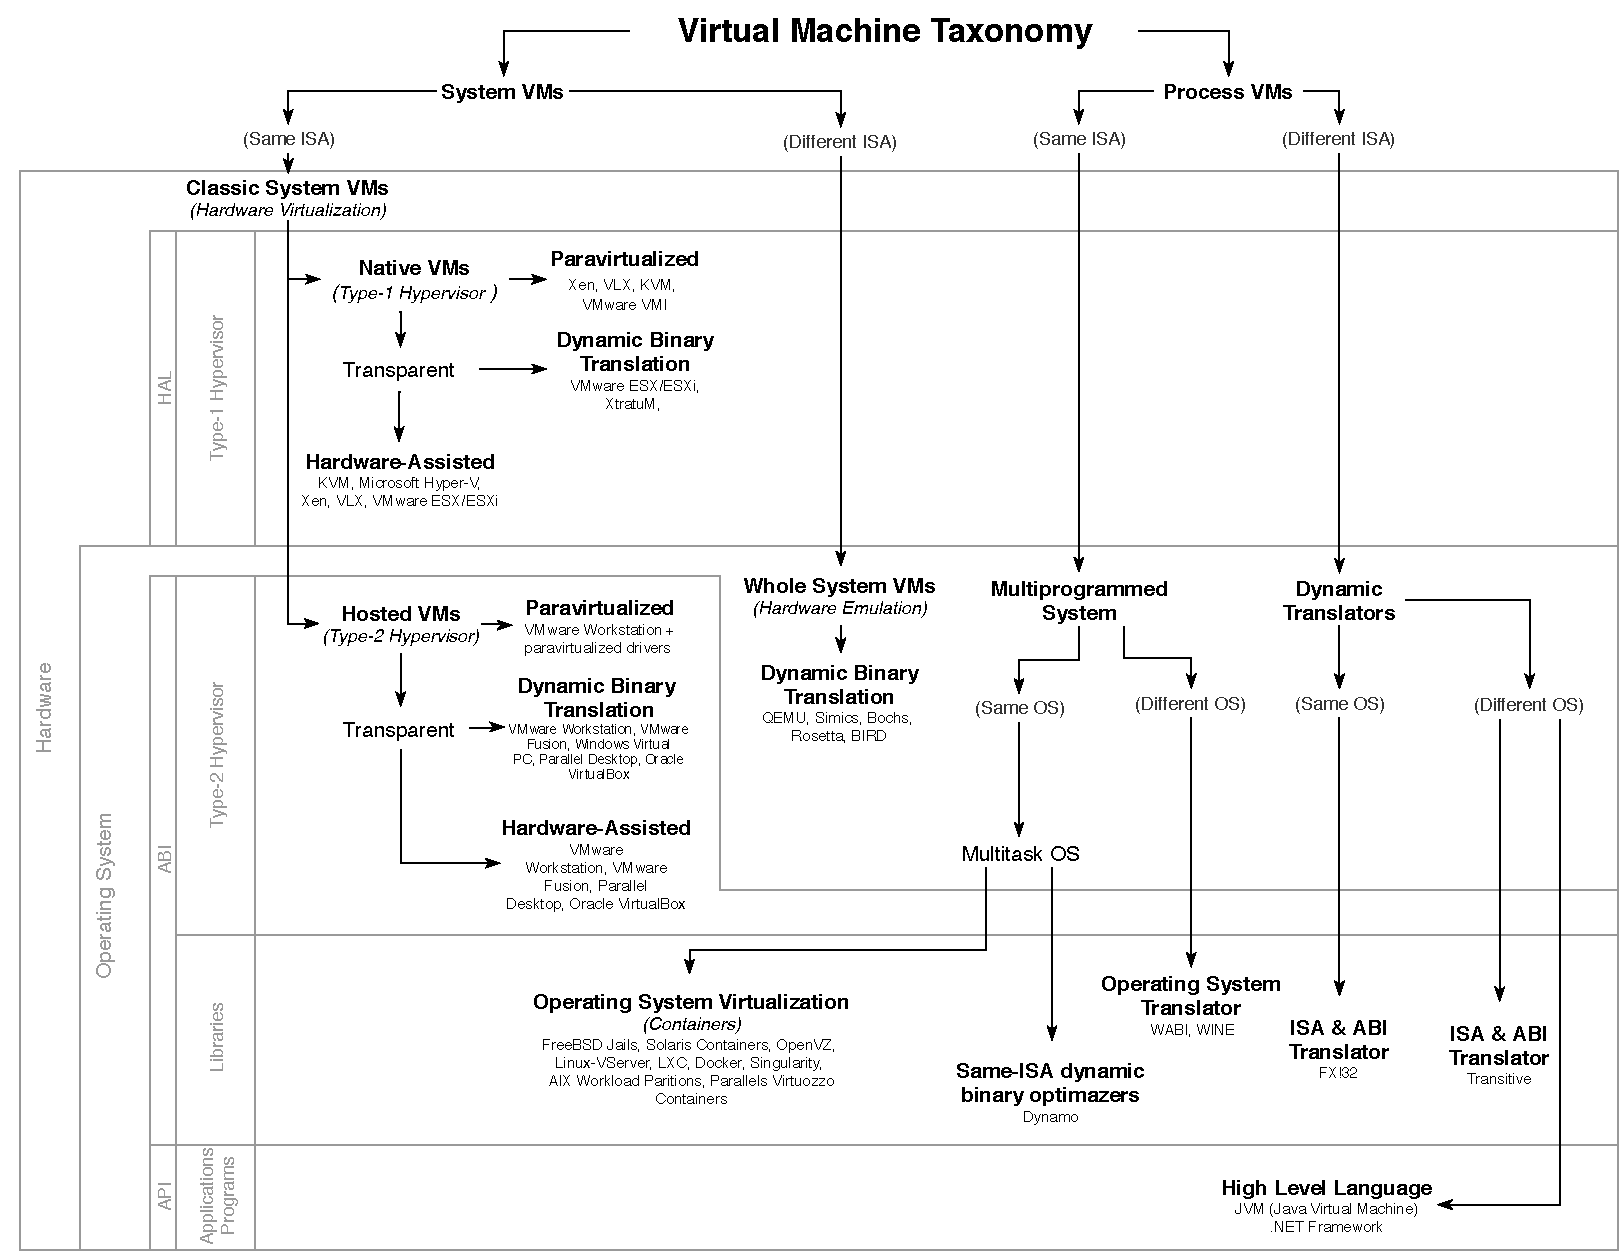
\includegraphics[width=17cm]{images/virtualMachineTaxonomy.pdf}
		\vspace{-0.2cm}%
		\caption{Virtual Machine Taxonomy Proposal. This taxonomy shows the outdated names of virtualization technologies that have lost validity. However, these names are still used to help the community to understand the positions within this new taxonomy. It is also important to include virtualization technologies that have gained full recognition in the industry and academia, such as \textit{Docker} and \textit{Singularity} among others. }
    	\label{fig:TaxonomiaPropuesta}
	\end{figure*}
	
	Starting from the concept of taxonomy as the science of naming things and classifying them into different groups \cite{CambridgeDictionary2018, Chi2000}, the taxonomic proposal technologies related to VMs is presented below. According to \textit{Chiueh} \cite{Chiueh2005} and \textit{Hoopes} \cite{Hoopes2009}, virtualization can occur either by aggregation (many elements are seen as one) or by a division of resources (one element looks like many). It is essential to clarify this point, as the taxonomy proposed in this paper focuses on aspects related to virtualization by \textit{resource division}. We also focus on server virtualization. We recommend that classifications of resource aggregation be kept separate from classifications of resource division. We note that studies like Kampert, Kusnetsky and Ameen which consider other types of virtualization do little to break down categories other than server/CPU virtualization. Thus we recommend that classifications of types of virtualization be kept separate from classifications of how server/CPU virtualization is implemented.  
	
	
	%JNM Say a bit more clearly why you are rejecting Kusnetsky and Kampert?  Mention Pessolani specifically too.. you are keeping that one also yes?
	
	%We chose not to include the taxonmies of Kusnetsky and Kampert because they are including virtualization of other kinds of resources like storage and networking. 
	%Also give the reader a heads up on that earlier in the paper.. when you introduce them 
	%say they are worth mentioning but beyond your scope in this paper or something like that
	
	%LESR new
	
Our proposed taxonomy, focused on resource division and server/CPU virtualization, builds based on the twelve reviewed studies, but is particularly focused on the studies such as that made by \textit{Chiueh} in 2005 \cite{Chiueh2005}, \textit{Smith and Nair} in 2005 \cite{Smith2005}, \textit{SCOPE Alliance Virtualization Group} in 2008 \cite{SCOPEAlliance2008}, \textit{P{\'e}k et al.} in 2013 \cite{Pek2013} and \textit{Bugnion et al.} in 2017 \cite{Bugnion2017}.
	
	Our taxonomy integrates the taxonomic approaches \textit{Level of abstraction} and \textit{Type of VM}. The first approach is oriented towards the use of layers, based on the levels of abstraction of the classical architecture of a computer system. The second approach is oriented towards the types of virtual machines that are either system or process. See Figure \ref{fig:TaxonomiaPropuesta}. 
	
	% Old
	%The \textit{Virtualization domains} approach was not considered in the present taxonomy.  This because some of the identified domains represent an interesting bet in the effort to organize elements or technological resources related to virtualization, but these are outside of the definition of virtualization made by \textit{Goldberg} \cite{Goldberg1973}, which is the approach followed in this paper. Therefore, in this taxonomic proposal, the integration of the \textit{Abstraction Level} and \textit{Virtual Machine Type} approach aims to present a way of visualizing the virtualization technologies related to VMs. This taxonomy allows the simultaneous display of the type of VM and its respective level of abstraction. The following sections, set out the taxonomy approaches contained in this proposal.
	
	%LESR new
	
	%The virtual machine taxonomy proposed here seeks to maintain consistency with the theoretical principles established in the definition of virtual machine given by Popek \cite{Popek1974} and Goldbert \cite{Popek1974, Popek1974}. In this sense, the domains "Type of VM" and "Level of abstraction" fit properly, however, the Domains of virtualization approach does not do it completely. This is why some categories of work using this approach will not be taken into account for inclusion in this proposal. For example, the security and administration and desktop domains described in Kampert's work; the access and administration categories of Kusnetzky's study and the Resource, grid and cloud virtualization categories of Abdulhamid's work, among others. 
	
	
	
	\subsection{Taxonomic Dimension 1: Abstraction level}

	This approach is based on the use of labels to determine layers similar to the levels of abstraction of a computer system, such as: Hardware, HAL, Operating System, ABI, API, Type-1 hypervisor, Type-2 hypervisor.   In Figure \ref{fig:TaxonomiaPropuesta}, the labels correspond to the levels of abstraction that are located on the left side. They also form the title of the rectangular structures with the horizontal distribution of the taxonomy. These rectangular structures identify a layer for the technologies contained in them.
	
	With the use of these layers, the taxonomy makes it possible to locate virtualization technologies depending on the level at which they take place. Thus, the reader can quickly infer aspects such as the dependence or not of an underlying OS and also determine the number of intermediaries involved in the virtualization process. This therefore allows us to infer in some occasions, the possible performance of these technologies.
	
	With regards to the HAL layer, the presence of a Type-1 hypervisor category can be seen. It also makes hardware-assisted virtualization technology visible in architectures such as x86. Both labels show that this type of hypervisor is directly placed over the hardware.  This arrangement is called \textit{bare-metal} and it is identified by the absence of intermediaries between the VMs and the hardware, which suggests a higher performance for the set of technologies located in this layer.
	
	The layer corresponding to the OS shows other technologies that apply virtualization through the presence of independent Type-2 hypervisors, or in conjunction with the technologies that assist virtualization from the hardware. This layer also indicates that virtualization is carried out through ABI using calls to the OS and using the latter as an intermediary between host systems and hardware. This situation suggests that the virtualization technologies belonging to this layer may present an inherent degradation in performance due to the costs of intermediation between the different environments.
	
	In the same layer, its also shows that there are virtualization technologies based on segmenting the OS in light operational environments, currently known as containers. To a large extent, they can contrast performance degradation because they do not perform virtualization of a complete OS.
	
	The last level of abstraction shows virtualization technologies that use APIs as a base. In the case of high-level languages, these can offer a high level of portability because generally, the APIs are used for multiple hardware and software platforms.
	
	\subsection{Taxonomic Dimension 2: Type of VM}
	
	First, VMs are considered as \textit{System VMs} or \textit{ Processes VMs}. 
	
	%In Figure \ref{fig:TaxonomiaPropuesta}, this approach corresponds to the interpretation of \textit{top-down}.
	
 \textit{System VMs} contain within their virtual environment a complete OS (guest OS) while \textit{Process VMs} do not. Instead, Process VMs use the \textit{host} OS as an intermediary between the virtual environment and the real hardware. A description of each category follows.
 
 Notice that some specific products appear in more than one category when they offer different modes of operation.
	
	\subsection{System VMs}
	
	The \textit{System VMs} are divided into two categories.  The first category is called \textit{Classic System VMs} where both host and guest use the same ISA. The second category is called \textit{whole system virtual machines} where the host and guest use different ISA.
	
	\subsubsection{Classic system VMs} This type of virtualization is also known as \textit{Hardware Virtualization}, and in turn includes two categories, the first one is called \textit{Native VMs} and the second one \textit{Hosted VMs}. It is important to note that each of these categories takes place at different levels of abstraction.
	
	\textbf{Native VMs}: This category is also known as \textit{Type-1 Hypervisors} and corresponds to the HAL abstraction level. Its characteristic is using a software layer directly on top of the hardware. It also presents a subdivision as shown below:
		
	\begin{list}{$\bullet$}{\setlength{\leftmargin}{5pt}}

			\item \textbf {Transparent} refers to VMs whose guest OS is not aware of their virtualization status and can finally be classified as \textit{Hardware-assisted} or \textit{dynamic Binary Translation}.
			
			\begin{list}{$\diamond$}{\setlength{\leftmargin}{8pt}}

				\item \textbf{Hardware-Assisted} virtualization involves the use of physical components to facilitate the management of virtual machines. This category includes examples such as KVM, Microsoft Hyper-V \cite{Kappel2009}, Xen, VLX and VMware ESX/ESXi \cite{VMware2018Website}.
				
				\item \textbf{Dynamic binary translation} implies that the Type-1 Hypervisor catches and inspects the code of each guest OS request to convert it into a proper request towards the underlying hardware. For examples VMware ESX/ESXi and XtratuM \cite{XtratuM}.
				 
			\end{list}
			
			\item \textbf{Paravirtualized} is also known as \textit{operating system-assisted virtualization} \cite{VMware2008}, \cite{VMware2018Website} and refers to efficient communication between the guest OS and the hypervisor. This implies modifying the guest OS to be aware of virtualization and to take advantage of that condition. This category includes examples, such as; Xen, VLX, KVM and VMware VMI \cite{VMware2018Website}.
			
		\end{list}	
	

	

\textbf{Hosted VMs} also known as \textit{Type-2 Hypervisors}, correspond to the ABI abstraction level. The main characteristic of this type of virtualization is using a layer of software on a pre-existing OS. Furthermore, it also presents a subdivision as shown below:
		
	\begin{list}{$\bullet$}{\setlength{\leftmargin}{5pt}}
		
			\item \textbf{Transparent} refers to VMs whose guest OS is not aware of their virtualization status. These virtual machines are classified in \textit{Hardware-Assisted} or \textit{Dynamic Binary Translation}.
			
			\begin{list}{$\diamond$}{\setlength{\leftmargin}{8pt}}

				\item \textbf {Hardware-Assisted} involves the use of physical components to facilitate the management of virtual machines. This category includes examples, such as VMware Workstation, VMware Fusion, Microsoft Virtual PC, Parallel Desktop, and Oracle VirtualBox.
				
				\item \textbf{Dynamic Binary Translation} implies that the Type-2 Hypervisor catches and inspects the code of each of the guest OS's requests to convert it into a proper request towards the underlying hardware. Examples here include VMware Workstation, VMware Fusion, Microsoft Virtual PC, Parallel Desktop and Oracle VirtualBox.
				
%JNM - explain when a given example is listed under multiple categories.. review these.. are you sure they are all under both?


			\end{list}
			
			\item \textbf {Paravirtualized} refers to efficient communication between the guest OS and the Type-2 Hypervisor; which implies modifying the guest OS to be aware of virtualization and take advantage of that condition. An example of this category is VMware Workstation, with the addition of the corresponding paravirtualization \textit{driver} to the network in the guest OS \cite {VMware2018Website}.
			
		\end{list}	

	\subsubsection{Whole system VMs}
	This type of virtualization is also known as \textit{Hardware emulation} and takes place at the ISA abstraction level.  This emulation presents an ISA different from the underlying hardware. However, in the proposed taxonomy it is located at the ABI abstraction level, which makes evident the existence of a pre-existing OS on which emulation can occur.
	
	\subsection{Proccess VMs}
	
	The \textit{Process VMs}, as well as the \textit{System VMs}, present a division according to the ISA projected in the virtual environment. When the ISA is the same, the category is called \textit{multiprogrammed systems}; otherwise, the category is called \textit{Dynamic translators}. Both categories are initially located at the level of the OS. This indicates the dependence of a pre-existing OS with has the purpose of generating the virtual environment for the processes. Each of these categories and their respective derivations is described below.
	
	\subsubsection{Multiprogrammed systems}
	
	Multiprogrammed systems implement the ability to share the OS among many processes, generating independent execution spaces for each one. This generates the illusion that for a moment of time, a process is an exclusive executor in the system. This category is then divided into two depending on whether there is an OS. When the same OS is projecting, the category is called \textit{Multitasking OSs}; otherwise, they are called \textit{OS translators}.
	
	\textbf {Multitasking OS} is dividing in turn into \textit{OS virtualization} and \textit{Same-ISA dynamic binary optimizer}, which are described below:
		
	\begin{list}{$\bullet$}{\setlength{\leftmargin}{5pt}}
	
		\item \textbf{Operating System Virtualization}: Applies at the ABI abstraction level, and uses system calls for interaction with the underlying hardware. It uses the pre-existing OS, and through isolation mechanisms it allows the generation of independent workspaces for the processes. Currently, this type of virtualization is booming and is often known as \textit {lightweight virtualization}, \textit{container-based virtualization} or simply \textit{containers}. The following examples stand out in this category: FreeBSD Jails \cite {Biederman2006}, Solaris Containers \cite {SolarisZones}, OpenVZ \ cite {OpenVZ}, Linux-VServer \cite {Linux-VServer}, AIX Workload Partitions (WPAR) \ cite {WPAR}, Parallels Virtuozzo Containers \cite {Virtuozzo}, LXC \cite {LXC}, Docker \cite {Docker} and Singularity \cite {Sylabs.io}.
			
		\item \textbf{Same-ISA dynamic binary optimizers} are fully implemented translators in software which perform optimized translations of binary code with an equal ISA. Its operation is completely transparent, and even the system's native binaries can be optimized too. An example of this category is the Dynamo project \cite{Bala2011}.
	\end{list}
		
	\textbf{Operating System Translator} allows the execution of applications built for OSs different from the system \textit{host}. For example, WINE \cite{Wine} and WABI \cite{WABI}.
		
	\subsubsection {Dynamic Translators}
	
	They rely on a pre-existing OS and support applications built for an ISA that is different from the system host's hardware. According to the differences between the \textit{host's OS} and \textit{guest's OS}, they are called \textit{ISA \& ABI Translator with the same OS}. FX!32 is an example if the host's OS and guest's OS are the same \cite{Chernoff1998}. In the opposite case, the category is called \textit{ISA \& ABI Translator with a different OS}. For example, JVM and .NET Framework.
	

    \section {Taxonomic-key diagram}           \label{sec:choosingVirtualizationTechnology}
	\begin{figure*}[ht]
		\centering
		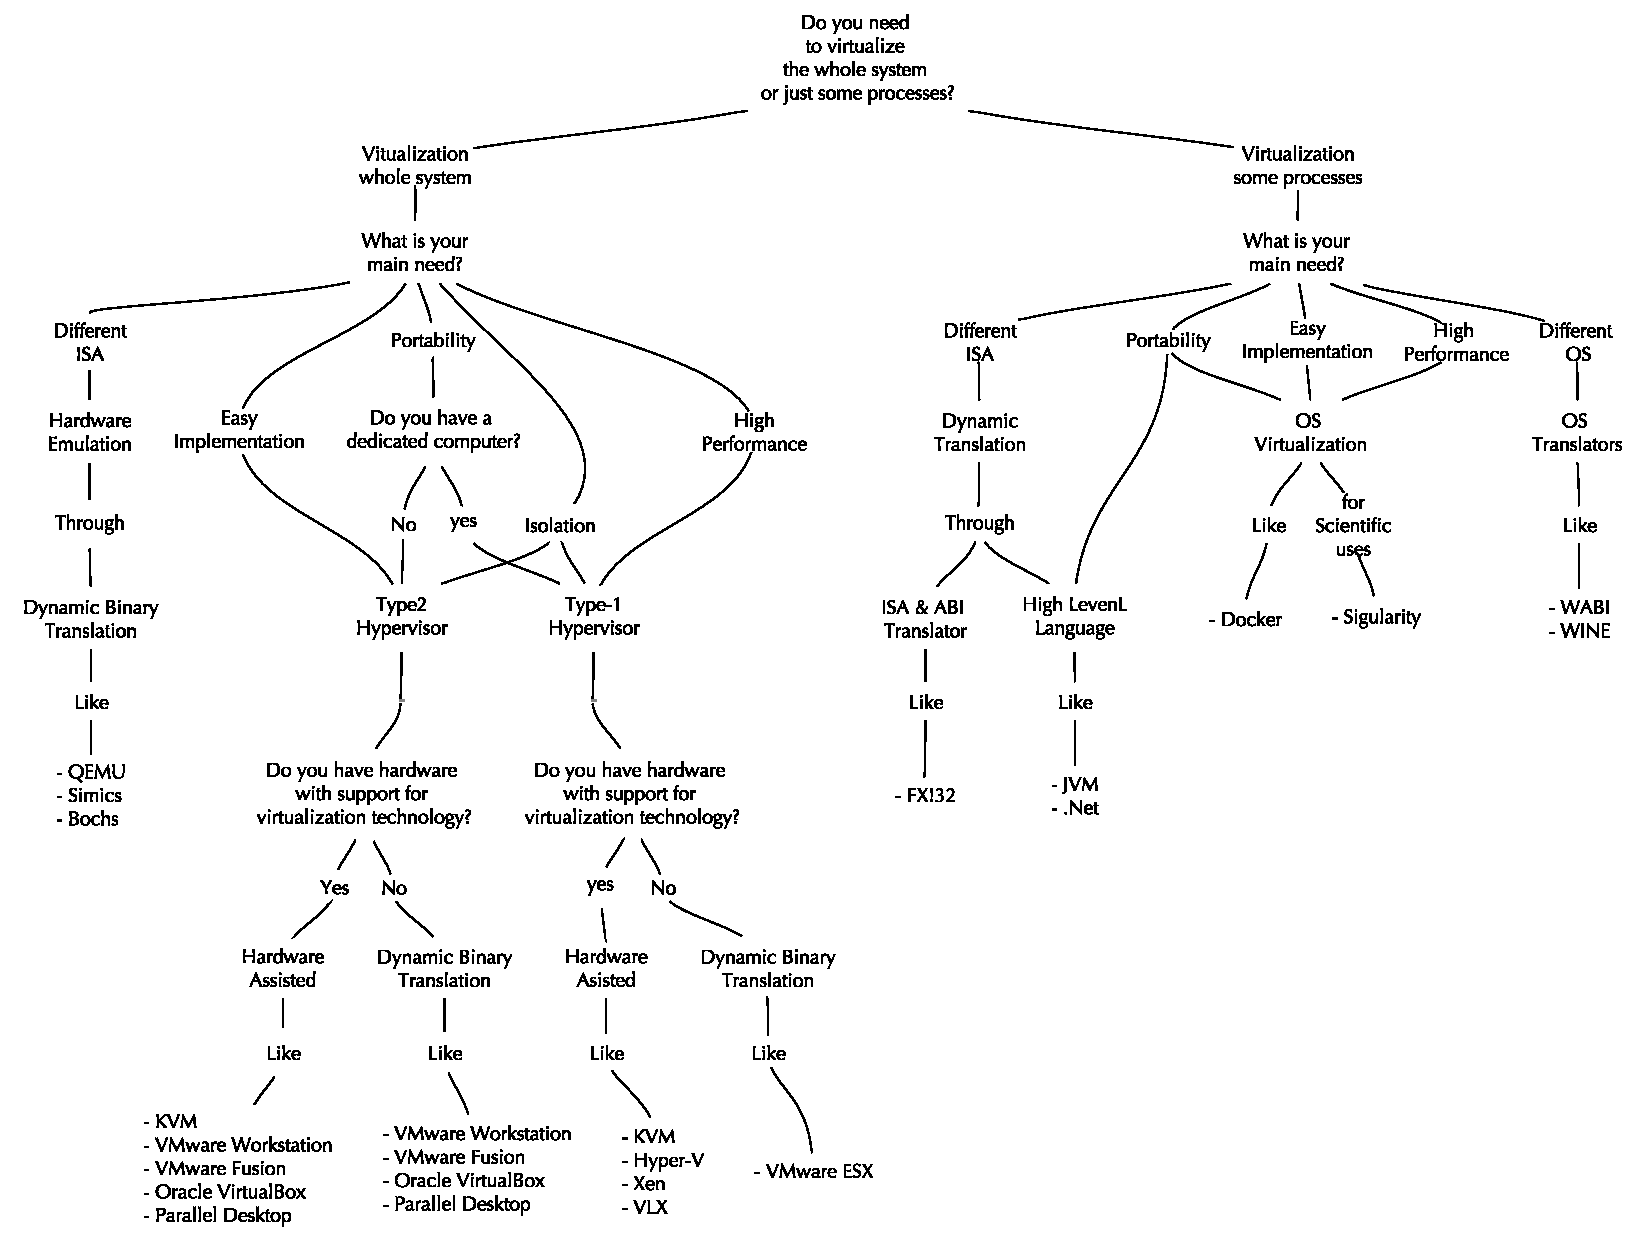
\includegraphics[width=18cm]{images/taxonomic-KeyDiagramV2.pdf}
		\vspace{-0.2cm}
		\caption{Taxonomic key diagram for the selection of virtualization technologies.}
		\label{fig:taxonomic-keyDiagram}
	\end{figure*}
	
	In this paper, we also propose a second element that consists of a \textit{taxonomic-key diagram}, similar to the dichotomous keys used in Biology. The purpose of this diagram is to decision making about the technologies related to the virtual machines indicated in the proposed taxonomy, see Figure \ref{fig:taxonomic-keyDiagram}. The diagram uses a set of questions, which, depending on each possibility of response, it establishes a path that leads to the identification of a type of virtual machine technology defined in the previous taxonomy. For example, the diagram can be interpreted by asking the question, Do you need to virtualize the entire system or just some of its processes? If the complete system needs to be virtualized, the following question will inquire about the specific need. If the desired virtual system needs an ISA different from the underlying hardware, the answer from the taxonomic-key is set the category \textit {Dynamic Binary Translation}, for example; \textit{QEMU}, \textit{Simics} and \textit{Botch}. As shown in the previous example, the result of the taxonomic key can be diverse and is subject to each possible response.

    	\section {Conclusions}\label{sec:conclusion}
	
	This paper present the following contributions:  
	
	\begin{list}{$\bullet$}{\setlength{\leftmargin}{5pt}}
	
	    \item A review of literature about the different classification schemes that have emerged in virtualization technologies has been carried out. These schemes have been introduced using a timeline that has allowed the identification of following taxonomic approaches \textit{Abstraction Level}, \textit{Virtual Machine Type} and \textit{Virtualization Domains}.
		
		\item When performing the analysis of each classification scheme, it was possible to identify particular weaknesses. These include; the presence of a single taxonomic approach in each scheme, and the lack of topicality considering the date of publication, and the absence in the details of the inclusion of technologies.
		
		\item The proposed taxonomy responds to the needs identified in the classification schemes analyzed. As a result, the proposal combines the \textit{Abstraction Level}, and \textit{Virtual Machine Type} approaches, giving the reader a means of visualizing the virtualization technologies relating to virtual machines. By doing so, the reader is always aware of the level of abstraction in which each technology takes place, in addition to the type of machine projected, be it a complete system or an execution environment for processes.
		
		\item The proposed taxonomy can be used in the academic field as a tool to facilitate teaching and learning processes in the academic community with interests in this type of technology, or in the business field to favour decision making when they need to implement technologies related to virtual machines. 
		
		\item Taxonomy allows the classification of virtualization technologies that are present in more than one conceptual branch, since these tools evolve meeting the needs of more than one approach by themselves, or use extensions to do so.
		
		\item Finally, a taxonomic-key diagram has been created for use by the industry as a tool to help when selecting virtualization technologies according to their different needs.

	\end{list}


    \bibliographystyle{unsrt}
    \bibliography{bibliography}

\label{last-page}
\end{multicols}
%\label{last-page}
\end{document}

